\documentclass[12pt,leqno]{article}
\usepackage[a4paper,margin=1in]{geometry}
\usepackage{lmodern}
\usepackage[T1]{fontenc}
\usepackage[leqno]{amsmath}
\usepackage{amssymb,amsthm}
\usepackage{booktabs,threeparttable}
\usepackage{graphicx}
\graphicspath{{figures/}}
\usepackage{setspace}
\usepackage[round,authoryear]{natbib}
\usepackage{caption}
\usepackage{float}
\usepackage{microtype}
\usepackage[hidelinks]{hyperref}

\captionsetup{font=small,labelfont=it,justification=justified,singlelinecheck=false}
\onehalfspacing
\setlength{\parskip}{0pt}
\setlength{\parindent}{1.5em}

% Float placement: keep exhibits beside the text that first cites them.
\setlength{\textfloatsep}{12pt plus 2pt minus 2pt}
\setlength{\floatsep}{12pt plus 2pt minus 2pt}
\setlength{\intextsep}{12pt plus 2pt minus 2pt}
\renewcommand{\topfraction}{0.92}
\renewcommand{\bottomfraction}{0.85}
\renewcommand{\textfraction}{0.06}
\renewcommand{\floatpagefraction}{0.90}
\setcounter{topnumber}{3}
\setcounter{bottomnumber}{2}
\setcounter{totalnumber}{4}

% AEA sectioning: Roman sections, lettered subsections, unnumbered introduction.
\renewcommand{\thesection}{\Roman{section}}
\renewcommand{\thesubsection}{\Alph{subsection}}

\newtheorem{proposition}{Proposition}
\newcommand{\pending}[1]{\textbf{[[#1]]}}

\title{Automation Exposure and the UK Labour Market: Employment, Pay and the Wage Floor, 2014--2020\thanks{Zhu: Oxford Internet Institute, Stephen A. Schwarzman Centre for the Humanities, University of Oxford, Radcliffe Observatory, Woodstock Road, Oxford OX2 6GG, United Kingdom (email: yiven.zhu@oii.ox.ac.uk). This paper is sole-authored. It develops coursework supervised and marked by Professor Roland Kappe of University College London, whose comments on the choice of cut-off, the assessment of pre-trends and the scope for placebo tests set the agenda for this revision. An anonymous reviewer for the \emph{UCL Journal of Economics} identified the collinear time specification, the composition concern and the confound with the National Living Wage, and proposed the floor-exposure design estimated in Section~\ref{sec:results}. No funding was received for this research and the author has no competing interests to declare. The research uses published aggregate statistics only and involves no human subjects, so no ethics review was required. Large language model tools assisted with reference checking and the appendices. The author reviewed all of it and takes full responsibility for the content. Replication materials are described in Appendix~\ref{app:repro}. All errors are mine.}}
\author{Louis Yiven Zhu}
\date{September 2026}

\begin{document}
\maketitle

\begin{abstract}
\noindent Occupations that the Office for National Statistics rated more automatable lost employment after 2016 and gained relative pay. Joining the ONS automation probability to seven Annual Survey of Hours and Earnings releases for 366 UK occupations, log employee jobs fall by 0.483 log points per unit of probability, with a break at 2016 and a pre-period coefficient of the opposite sign. Mean pay rises by 0.122 along a path that begins before 2016 and that exposure to the National Living Wage accounts for. Estimating the pay margin alone reverses the sign of the labour-market story.
\end{abstract}

\noindent \emph{JEL codes:} J23, J24, J31, J38, O33 \\
\emph{Keywords:} automation exposure, occupational employment, occupational wages, minimum wage, event study, United Kingdom

\bigskip

Whether technologies that can perform an occupation's tasks reduce employment or pay in that occupation is the central empirical question of the task-based literature. The first years of commercial deep learning offer a window in which to ask it of artificial intelligence (AI) with the exposure measure a national statistical agency itself publishes. Task-displacement models predict that occupations whose tasks capital can take over lose labour demand, and the loss shows up as lower relative employment or lower relative pay depending on how wages adjust \citep{acemoglu2019automation, acemoglu2022tasks}. The evidence on pay in AI-exposed occupations is thinner than the theory. \citet{acemoglu2022vacancies} find that AI-exposed US establishments cut non-AI hiring after 2010, with effects on employment and wages in exposed occupations too small to detect in aggregate, and \citet{webb2020impact} reports declines in employment and pay for occupations exposed to the earlier automation technologies, software and industrial robots. This paper asks the question for the United Kingdom, follows employment and pay together, and finds that the two margins tell opposite stories unless the wage floor and the composition of occupations are held fixed.

The setting joins two public series on one classification. The Office for National Statistics (ONS) assigns each four-digit occupation in the Standard Occupational Classification 2010 (SOC 2010) a probability of automation, built with the method of \citet{frey2017future} and published in 2019 on 2017 task data \citep{ons2019automation}. The Annual Survey of Hours and Earnings (ASHE) publishes, for the same occupations, mean and median gross hourly pay, the number of employee jobs, paid hours, and a set of pay percentiles each April \citep{ons2024ashe}. Joining them yields 2,546 occupation-year cells for 366 occupations across the 2014 to 2020 releases, the seven releases ASHE published on SOC 2010. A working-paper version of this analysis extended the panel to 2023 and read a positive post-2016 interaction between the probability and pay as support for an augmentation account. This version restricts the panel to a single classification, adds employment and hours, builds the exposure to the National Living Wage (NLW) that a reviewer of that version asked for, and reaches a different conclusion.

The employment result is the paper's main finding. On the 309 occupations with a published jobs count in every release, log employee jobs regressed on the probability interacted with a post-2016 indicator returns $-0.483$ under occupation and release fixed effects (standard error 0.057, clustered by occupation). An occupation one standard deviation more automatable, where the standard deviation of the probability is 0.145, therefore had employment about 7.0 log points lower after 2016 relative to before, or 6.8 per cent. The event study places the movement in time. Relative to 2015, the 2014 coefficient is $+0.095$ (0.044), so more automatable occupations were gaining employment before the treatment date. The coefficients then run $-0.243$, $-0.245$, $-0.324$, $-0.494$ and $-0.869$ from 2016 to 2020. Aggregate employment in the balanced panel grew from 24.7 to 26.5 million jobs over 2014 to 2019, while the share of those jobs in above-median-risk occupations fell from 54.1 to 50.8 per cent, so the pattern is reallocation across occupations within a growing total. Conditioning on the occupation's exposure to the NLW leaves the estimate at $-0.536$ (0.072).

Pay moved the other way, and the movement is explained by the wage floor. The same interaction for log mean gross hourly pay is $0.122$ (0.019), or 1.8 per cent per standard deviation of the probability. The event study shows that the pay gradient in 2014 was 0.043 log points lower than in 2015 (0.017), an increment as large as the 0.051 (0.014) gain from 2015 to 2016, and that it then rose by between 0.023 and 0.051 log points in each release to 2019. A regression that allows the gradient to trend linearly and adds a 2016 break returns a trend of 0.034 per year (0.007) and a break of 0.015 (0.020) over 2014 to 2019. The share of an occupation's jobs paid below \pounds 7.20 in the 2015 release measures its exposure to the NLW rate of April 2016. Interacting that share with the post-2016 indicator lowers the pay coefficient from 0.132 (0.018) to 0.033 (0.021), and allowing the share its own path in every release leaves the pay event-study coefficients for 2016 to 2020 at $-0.002$, $0.003$, $0.023$, $0.051$ and $0.005$, none distinguishable from zero.

Read together, the two margins describe an occupational labour market in which more automatable occupations shed jobs after 2016 while a rising floor and the exit of the lowest-paid jobs lifted the pay of those who remained. Appendix~\ref{app:theory} sets out a framework in which a demand shift against automatable tasks, a binding wage floor and a within-occupation pay distribution produce exactly this pattern. It derives the share of jobs below the floor as the first-order effect of a floor increase on occupational mean pay, and it records one prediction the data do not support. The reader should not take the employment finding for a causal estimate of automation. The design has no measure of technology adoption, and the probability is a 2017 assessment of task automatability that predates large language models. The design can establish that the probability predicts relative employment loss after 2016 with no pre-trend of the same sign, that it predicts faster relative pay growth only through the level of pay, and that the two facts are consistent with a single account.

The paper's contribution is therefore threefold. It documents the joint evolution of employment and pay across UK occupations ranked by a published automation probability over 2014 to 2020. It shows that an exposure-score difference-in-differences with a single post period, estimated on pay alone, recovers a pre-existing compression driven by the wage floor and reverses the sign of the labour-market story. It also documents in Section~\ref{sec:soc} and Appendix~\ref{app:soc} that joining releases published on SOC 2020 to SOC 2010 risk scores by numeric code attaches the score to a different occupation for 125 of 261 matched codes, and that this mismatch manufactured the largest coefficients in the earlier version. The second and third points transfer to any application of an occupation-level exposure score to a national pay series.

The analysis answers three questions. \textbf{RQ1} asks whether the cross-occupation gradient between the automation probability and log pay changed after 2016, and whether the change is a break at 2016 or the continuation of a trend that predates it. \textbf{RQ2} asks how much of the pay movement is accounted for by exposure to the National Living Wage. \textbf{RQ3} asks whether employment and hours in more automatable occupations changed after 2016, and with what timing. Section~\ref{sec:lit} places the question in the task-based, exposure-score and minimum-wage literatures. Section~\ref{sec:data} describes the panel and the exposure measure. Section~\ref{sec:strategy} sets out the specifications and states what each identifies. Section~\ref{sec:results} answers the three questions by name. Section~\ref{sec:sens} reports alternative specifications. Section~\ref{sec:soc} reports the classification join. Section~\ref{sec:discussion} states the limitations in decreasing order of consequence.

\begin{figure}[!ht]
\centering
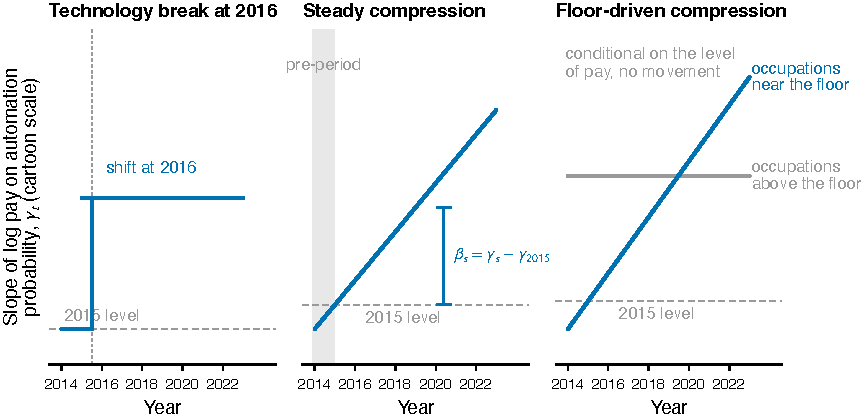
\includegraphics[width=0.98\textwidth]{fig1_concept.pdf}
\caption{Three accounts of a rising automation-risk gradient of pay. The cross-occupation slope of log pay on the ONS automation probability, $\gamma_t$, is negative in every year because automatable occupations pay less. A technology break (Panel A) implies that $\gamma_t$ is flat before 2016 and shifts after it. A steady compression (Panel B) implies a straight line through the pre-period, so a post-2016 indicator picks up the trend. A floor-driven compression (Panel C) implies that the movement in $\gamma_t$ comes from occupations near the wage floor and vanishes once exposure to the floor is held fixed. The event studies in Section~\ref{sec:results} estimate $\beta_s = \gamma_s - \gamma_{2015}$ for pay and for employment in each release and adjudicate among the three for each margin. The panels carry cartoon data and no estimates.}
\label{fig:concept}
\end{figure}

\section{Automation Exposure, Wage Floors and the UK Setting}\label{sec:lit}

The question sits at the intersection of three literatures, and the gap this paper fills is the join between the first and the third on a national pay series with both quantity and price margins. The task-based tradition established that when capital acquires tasks previously performed by workers, automation reduces the labour share in value added and can reduce labour demand unless new tasks are created \citep{acemoglu2019automation}. The reduction in demand then shows up as lower relative pay in the occupations that lose tasks \citep{acemoglu2022tasks}. \citet{acemoglu2020robots} estimate that one additional industrial robot per thousand workers lowered wages in exposed US commuting zones by 0.42 per cent, alongside a fall of 0.2 percentage points in the employment-to-population ratio, over the 1990 to 2007 exposure window. \citet{graetz2018robots} find productivity gains from robots across 17 countries, with some reduction in the employment share of low-skilled workers. The routine-biased hypothesis of \citet{autor2003skill} gives the mechanism a task content, since computers substitute for codifiable routine tasks and complement non-routine analytic ones. This tradition predicts that exposure lowers both employment and pay in the affected occupations. It does not pose the question of how the two margins separate when the exposure measure is a published probability and the pay series sits under a binding statutory floor.

A second strand builds measures of exposure to AI specifically, and this paper borrows its measurement logic while taking no position on its contested pay findings. \citet{felten2021occupational} construct and validate the AI Occupational Exposure index, which links advances in AI to the abilities an occupation draws on. \citet{webb2020impact} constructs exposure from the overlap between patent text and occupational task descriptions and finds that occupations highly exposed to the earlier automation technologies saw declines in employment and pay. \citet{acemoglu2022vacancies} use the near-universe of US online vacancies to show that AI-exposed establishments reduced non-AI hiring after 2010, with aggregate effects on employment and wages in exposed occupations too small to detect. \citet{eloundou2024gpts} rate 1.8 per cent of US jobs as having more than half their tasks affected by large language models with simple interfaces, and 46 per cent once complementary software is allowed for, an exposure profile that rises with pay. The field experiment of \citet{brynjolfsson2025generative} finds that a generative-AI assistant raised the productivity of customer-support agents by 15 per cent, with gains concentrated among less experienced workers. None of these studies uses a UK exposure measure or a UK pay panel, and none follows employment and pay in the same occupations across a period in which a statutory floor rose.

The ONS probability itself belongs to the exposure-score family and carries two known limits. It descends from the method of \citet{frey2017future}, who assigned 702 US occupations a probability of computerisation from expert classification of task bottlenecks. \citet{arntz2017revisiting} showed that moving the classification from occupations to individual jobs reduces the share of US jobs at high risk from 38 to 9 per cent, because workers specialise in tasks within an occupation that differ in how automatable they are. The ONS measure also predates large language models, so it measures the automatability of 2017 tasks by the capabilities anticipated then. Both limits attenuate any technology signal in the probability, and neither removes its strong correlation with the level of pay, which is the property that this paper has to confront.

A third strand studies the UK wage floor. The NLW, introduced in April 2016 at \pounds 7.20 for workers aged 25 and over with a target of 60 per cent of median pay by 2020, raised the floor by 7.5 per cent at introduction and by between 4.2 and 6.2 per cent in each subsequent April to 2020. \citet{giupponi2024minimum} exploit geographic variation in exposure to the national floor and find a substantial rise in pay at the bottom of the distribution with spillovers up to roughly the twentieth percentile, and no statistically detectable fall in employment over 2016 to 2019. Because pay at the bottom of the distribution belongs disproportionately to occupations the ONS rates as automatable, any occupation-level pay series will register the floor as faster growth in high-risk occupations. \citet{autor2023compression} document the same compression in the United States after 2020 with no change in the federal floor, driven by tightness in the low-wage labour market and rising job-to-job separations. The minimum-wage literature does not ask what its findings imply for exposure-score studies of automation, and it does not ask whether the occupations most exposed to the floor were also the occupations losing employment for other reasons. This paper asks both.

The econometric point that joins the strands is now standard. \citet{roth2023trending} recommend that a static difference-in-differences estimate be accompanied by event-study estimates and pre-trend evidence that show when the outcome moves and whether it was already moving. \citet{callaway2024continuous} show that with a continuous treatment the two-way fixed-effects interaction identifies an average causal response only under a strong parallel-trends assumption, which rules out selection into dose on the basis of the path an occupation would follow. The ONS probability is a continuous dose that is correlated with the level of pay, and the level of pay determines exposure to the floor, so the strong assumption fails for the pay outcome by construction unless the floor is held fixed. The design below therefore reports every static interaction as a description, tests its timing, and conditions on a predetermined measure of floor exposure.

\section{Data}\label{sec:data}

The panel combines the ONS automation probability with five series from ASHE Table 14, all on the SOC 2010 four-digit classification and all for the 2014 to 2020 releases. ASHE samples 1 per cent of employee jobs from HM Revenue and Customs PAYE records with an April reference date. Table 14.5a reports, for each occupation, the number of employee jobs in thousands, the median and mean of gross hourly pay, and the 10th, 20th, 25th, 30th, 40th, 60th, 70th, 75th, 80th and 90th percentiles. Table 14.6a reports the same for hourly pay excluding overtime and Table 14.9a for total paid hours per week. Appendix~\ref{app:data} lists the workbook used for every release and the number of cells each publishes. Cells whose estimate the ONS suppresses for quality or disclosure are missing, and no cell is imputed.

The primary pay outcome is $\ln w_{it}$, the log of nominal mean gross hourly pay in occupation $i$ and release $t$. Pay is nominal throughout. Every specification includes release fixed effects, and a common deflator enters log pay additively by release, so nominal and real specifications return identical interaction and event-study coefficients, as Proposition~\ref{prop:deflator} shows. The median and the overtime-exclusive mean serve as alternative pay outcomes. The employment outcome is $\ln N_{it}$, the log of employee jobs, and the hours outcome is the log of mean paid hours. The jobs count is published for fewer cells than pay because the ONS suppresses small counts, so the employment analysis rests on 346 occupations with any published count and on 309 with a count in every release.

The exposure measure is the ONS probability of automation, $A_i$, for 369 SOC 2010 unit groups \citep{ons2019automation}. The ONS applied the \citet{frey2017future} method to 2017 Annual Population Survey task data and reported that 7.4 per cent of jobs in England were at high risk, defined as a probability above 0.7. Waiters and waitresses, shelf fillers and elementary sales occupations sit at the top of the distribution and medical practitioners, higher-education teaching professionals and senior professionals of educational establishments at the bottom. Across the 366 occupations that match at least one pay cell, the probability ranges from 0.181 to 0.728 with a mean of 0.446 and a standard deviation of 0.145. It does not vary over time, so occupation fixed effects absorb it in levels and all identifying variation comes from its interaction with time.

Exposure to the wage floor is a predetermined occupation attribute built from the 2015 release. For each occupation the share of employee jobs paid below \pounds 7.20, the NLW rate that took effect in April 2016, is interpolated from the published percentiles of the 2015 release on the assumption that pay is distributed piecewise linearly between adjacent published percentiles. Appendix~\ref{app:data} gives the formula as equation (B1) and works two occupations through it by hand. The share can be computed for 347 occupations. It has a mean of 0.086 and a standard deviation of 0.145, it is zero for the lowest-paid tenth of the distribution of occupations and 0.286 at the ninetieth percentile, and it correlates 0.60 with the automation probability. A second measure, the Kaitz index, is \pounds 7.20 divided by the occupation's 2015 median hourly pay and correlates 0.82 with the probability. Both are fixed at their 2015 values so that exposure is measured before the floor took effect.

\begin{table}[!ht]\centering
\caption{The occupation-year panel by release, 2014--2020}\label{tab:sample}
\begin{threeparttable}\footnotesize\setlength{\tabcolsep}{3pt}
\begin{tabular}{lcccccc}\toprule
 & & \multicolumn{2}{c}{Mean log hourly pay} & \multicolumn{2}{c}{Cross-section gradient} & Share of jobs in \\
\cmidrule(lr){3-4}\cmidrule(lr){5-6}
Release & Occupations & Below-median & Above-median & Slope & (s.e.) & above-median risk (\%) \\ \midrule
2014 & 364 & 2.891 & 2.360 & -2.114 & (0.083) & 54.0 \\
2015 & 365 & 2.896 & 2.380 & -2.071 & (0.081) & 54.1 \\
2016 & 365 & 2.902 & 2.399 & -2.030 & (0.079) & 52.8 \\
2017 & 363 & 2.924 & 2.419 & -2.009 & (0.080) & 52.6 \\
2018 & 364 & 2.948 & 2.452 & -1.980 & (0.079) & 52.3 \\
2019 & 363 & 2.964 & 2.485 & -1.926 & (0.076) & 50.8 \\
2020 & 362 & 2.954 & 2.475 & -1.923 & (0.075) & 48.0 \\
\bottomrule\end{tabular}
\begin{tablenotes}\footnotesize
\item \emph{Notes:} Each row describes the occupations with a published mean gross hourly pay in that ASHE release on the SOC 2010 basis, of the 366 occupations in the panel. Log pay is the log of nominal mean gross hourly pay. The median automation probability across the 366 occupations is 0.468. The gradient is the slope from a cross-sectional regression of log pay on the automation probability in that release, with heteroskedasticity-consistent standard errors in parentheses. The final column is the share of employee jobs in above-median-risk occupations among the 309 occupations with a published jobs count in all seven releases.
\item \emph{Source:} ASHE Table 14, 2014--2020 releases, revised editions; ONS (2019) probability of automation.
\end{tablenotes}\end{threeparttable}\end{table}

Table~\ref{tab:sample} describes the panel release by release. Each release publishes a mean for between 362 and 365 of the 366 occupations, and 358 occupations have a mean in all seven releases. The cross-sectional slope of log pay on the probability is $-2.11$ (0.08) in 2014, so an occupation one standard deviation higher in the probability paid 31 log points less, and it rises monotonically to $-1.92$ (0.08) in 2020. The final column shows the share of employee jobs in above-median-risk occupations, which falls from 54.1 per cent in 2015 to 50.8 in 2019 and 48.0 in 2020. Both series are the objects the regressions below model, and both move before any estimation. Table~\ref{tab:desc} gives descriptive statistics for every variable.

\begin{table}[!ht]\centering
\caption{Descriptive statistics}\label{tab:desc}
\begin{threeparttable}\footnotesize\setlength{\tabcolsep}{3pt}
\begin{tabular}{lccccc}\toprule
Variable & N & Mean & S.D. & Min & Max \\ \midrule
\multicolumn{6}{l}{\emph{Panel A. Occupation-year cells, 2014--2020}} \\
Log mean gross hourly pay & 2,546 & 2.675 & 0.367 & 1.908 & 4.052 \\
Mean gross hourly pay (\pounds) & 2,546 & 15.61 & -- & 6.74 & 57.51 \\
Employee jobs (thousands) & 2,303 & 78.7 & -- & 4 & 1178 \\
Mean paid hours per week & 2,551 & 35.1 & -- & -- & -- \\
\addlinespace
\multicolumn{6}{l}{\emph{Panel B. Occupation-level attributes, fixed over time}} \\
Automation probability & 366 & 0.446 & 0.145 & 0.181 & 0.728 \\
Share of jobs below \pounds 7.20 in 2015 & 347 & 0.086 & 0.145 & 0.000 & -- \\
\bottomrule\end{tabular}
\begin{tablenotes}\footnotesize
\item \emph{Notes:} Pay is nominal. Jobs and hours are the published occupation totals and means from ASHE Tables 14.5a and 14.9a; the jobs count is published for fewer cells because the ONS suppresses small counts. The automation probability is defined on the SOC 2010 four-digit classification. The share of jobs below \pounds 7.20, the National Living Wage rate of April 2016, is interpolated from the published percentiles of the 2015 release by equation (B1); its tenth and ninetieth percentiles across occupations are 0.000 and 0.286, and it correlates 0.60 with the automation probability.
\item \emph{Source:} ASHE Table 14, 2014--2020 releases, revised editions; ONS (2019) probability of automation.
\end{tablenotes}\end{threeparttable}\end{table}

\section{Empirical Strategy}\label{sec:strategy}

The static specification interacts the probability with a post-2016 indicator in a two-way fixed-effects (TWFE) regression,
\begin{equation}\label{eq:twfe}
y_{it} = \alpha_i + \lambda_t + \beta \left( A_i \times \mathbf{1}[t \geq 2016] \right) + \varepsilon_{it},
\end{equation}
where $y_{it}$ is log pay, log jobs or log hours, $\alpha_i$ is an occupation fixed effect, $\lambda_t$ a release fixed effect, and $\varepsilon_{it}$ an occupation-year disturbance. The earlier version included a post-2016 main effect alongside the release effects. The two are collinear, and the estimation software resolved the collinearity by dropping a release indicator while retaining the main effect, so the reported release coefficients had no interpretable base. Equation~\eqref{eq:twfe} omits the main effect and defines 2015 as the base release, which leaves $\beta$ unchanged. Each occupation-year receives equal weight in the main estimates, so $\beta$ describes the average occupation, and employment-weighted estimates that describe the average worker are reported alongside. Standard errors are clustered by occupation, which allows arbitrary serial correlation within an occupation's seven observations across 366 clusters.

The coefficient $\beta$ is the change, from the pre-2016 releases to the post-2016 releases, in the cross-occupation slope of the outcome on the probability. Proposition~\ref{prop:static} shows that with equal weights and a balanced panel it equals the slope of a regression of each occupation's post-minus-pre mean change in the outcome on its probability, and that it equals the average of the post-period event-study coefficients minus the average of the pre-period ones. It is a description of how the gradient moved. \citet{callaway2024continuous} show that with a continuous treatment a TWFE interaction identifies an average causal response only under a strong parallel-trends assumption, which requires that the path an occupation would follow at any given dose does not depend on the dose it holds. The probability is correlated at $-0.80$ with the 2014 level of pay, and the level of pay governs exposure to the NLW, so the assumption fails for pay unless the floor is held fixed. The employment outcome faces the same concern in principle, since a rising floor can reduce employment where it binds, which is why the floor-exposure control is applied to both margins.

The event study replaces the single indicator with a full set of release interactions,
\begin{equation}\label{eq:es}
y_{it} = \alpha_i + \lambda_t + \sum_{s \neq 2015} \beta_s \left( A_i \times \mathbf{1}[t = s] \right) + \varepsilon_{it},
\end{equation}
so that $\beta_s$ is the change in the gradient between 2015 and release $s$. With only the 2014 release before the treatment date, the single pre-period coefficient $\beta_{2014}$ cannot support a formal test of parallel trends, as \citet{roth2023trending} note for short pre-periods. It can show whether the gradient was already moving before 2016 in the direction and at the rate it moved after, which is the comparison each margin needs. A second specification tests the same point in one parameter by letting the gradient trend linearly and adding a break,
\begin{equation}\label{eq:trend}
y_{it} = \alpha_i + \lambda_t + \gamma \left( A_i \times (t - 2015) \right) + \delta \left( A_i \times \mathbf{1}[t \geq 2016] \right) + \varepsilon_{it},
\end{equation}
where $\gamma$ is the annual movement in the gradient and $\delta$ any level shift at 2016 beyond the trend. Under a break $\delta$ is different from zero and $\gamma$ near zero; under a steady movement $\gamma$ is different from zero and $\delta$ near zero. Proposition~\ref{prop:restriction} states equation~\eqref{eq:trend} as a restriction on the event-study coefficients and explains why $\delta$ is the less precisely estimated of the two.

The third specification conditions on the floor. Let $F_i$ be the occupation's 2015 share of jobs below \pounds 7.20, demeaned across occupations, and let $P_t = \mathbf{1}[t \geq 2016]$. The specification is
\begin{equation}\label{eq:nlw}
y_{it} = \alpha_i + \lambda_t + \beta \left( A_i \times P_t \right) + \theta \left( F_i \times P_t \right) + \kappa \left( A_i \times F_i \times P_t \right) + \varepsilon_{it}.
\end{equation}
The coefficient $\theta$ captures post-2016 movement that varies with exposure to the floor, $\beta$ is the risk gradient's movement at mean exposure, and $\kappa$ tests whether the two exposures interact. Proposition~\ref{prop:floor} shows that the share of jobs below the floor is the first-order effect of a floor increase on an occupation's mean pay when the pay index and composition are held fixed, so the share is the appropriate regressor and its coefficient has a structural reading. An event-study version interacts $F_i$ with every release indicator so that the floor path is unrestricted, and the Kaitz index replaces $F_i$ as a check.

Inference uses standard errors clustered by occupation throughout. Because the treatment is a fixed occupation attribute, a permutation test that reassigns the 366 probabilities at random across occupations 2,000 times and re-estimates equation~\eqref{eq:twfe} gives the distribution of $\hat{\beta}$ under the null that the probability carries no information about the outcome's dynamics.

\section{Results}\label{sec:results}

\subsection{The Pay Gradient after 2016, and Whether It Broke or Trended}

Table~\ref{tab:pay} reports equation~\eqref{eq:twfe} for pay. On the 2014 to 2020 panel the interaction is 0.122 (0.019), with a 95 per cent confidence interval of $[0.085, 0.158]$. Multiplying by the occupation-level standard deviation of the probability of 0.145 gives 0.018 log points, so an occupation one standard deviation more automatable saw mean pay about 1.8 per cent higher after 2016 relative to before, conditional on occupation and release effects. The estimate is 0.124 (0.018) on the 358 occupations present in every release, 0.116 (0.018) on the 2014 to 2019 releases, 0.139 (0.019) with the median in place of the mean, and 0.124 (0.019) with hourly pay excluding overtime. Weighting by 2015 employee jobs raises it to 0.187 (0.025) against 0.134 (0.019) unweighted on the same 333 occupations, so the compression is stronger among large occupations. Across every pay definition the gradient became less negative after 2016, by an eighth of a log point per unit of probability.

\begin{table}[!ht]\centering
\caption{Post-2016 change in the automation-risk gradient of log hourly pay}\label{tab:pay}
\begin{threeparttable}\scriptsize\setlength{\tabcolsep}{2.5pt}
\begin{tabular}{lcccccc}\toprule
 & (1) & (2) & (3) & (4) & (5) & (6) \\
 & Mean pay & Balanced & 2014--19 & Weighted & Median pay & Excl.\ overtime \\ \midrule
Risk $\times$ post-2016 & 0.122 & 0.124 & 0.116 & 0.187 & 0.139 & 0.124 \\
 & (0.019) & (0.018) & (0.018) & (0.025) & (0.019) & (0.019) \\
95\% confidence interval & [0.085, 0.158] & [0.088, 0.161] & [0.082, 0.151] & [0.138, 0.236] & [0.101, 0.177] & [0.088, 0.161] \\ \addlinespace
Occupation-years & 2,546 & 2,506 & 2,184 & 2,329 & 2,496 & 2,544 \\
Occupations & 366 & 358 & 366 & 333 & 367 & 366 \\
Within $R^{2}$ & 0.029 & 0.032 & 0.035 & 0.172 & 0.046 & 0.031 \\
\bottomrule\end{tabular}
\begin{tablenotes}\footnotesize
\item \emph{Notes:} The dependent variable is the log of the stated pay measure and the specification is equation (1). All columns include occupation and release fixed effects. Standard errors clustered by occupation are reported in parentheses. Column 2 keeps the 358 occupations with a published mean in all seven releases. Column 4 weights each cell by the occupation's employee jobs in the 2015 release, on the 333 occupations with a published count; the unweighted estimate on that same sample is 0.134 (0.019). Column 5 uses the published median of Table 14.5a and column 6 the mean of Table 14.6a. All other columns weight each occupation-year equally.
\item \emph{Source:} ASHE Table 14, 2014--2020 releases, revised editions; ONS (2019) probability of automation.
\end{tablenotes}\end{threeparttable}\end{table}

Table~\ref{tab:espay} and Figure~\ref{fig:espay} place the movement in time and show that it did not begin in 2016. In column 1 the coefficient for 2014 is $-0.043$ (0.017), so the gradient was 0.043 log points steeper in 2014 than in 2015. The coefficients for 2016 to 2020 are 0.051 (0.014), 0.073 (0.020), 0.101 (0.023), 0.151 (0.024) and 0.125 (0.030). The year-on-year increments are 0.043 from 2014 to 2015, 0.051 from 2015 to 2016, then 0.023, 0.027 and 0.051, and $-0.027$ into 2020. The pre-treatment increment is indistinguishable in size from the treatment-year increment, and nothing in the sequence marks 2016 as the release in which the gradient began to move. The employment-weighted column 2 has the same shape at larger amplitude, with $-0.063$ in 2014 and 0.233 in 2020.

\begin{table}[!ht]\centering
\caption{Event-study estimates for log mean hourly pay, relative to 2015}\label{tab:espay}
\begin{threeparttable}\footnotesize\setlength{\tabcolsep}{3pt}
\begin{tabular}{lcccccc}\toprule
 & \multicolumn{2}{c}{(1) Unweighted} & \multicolumn{2}{c}{(2) Employment-weighted} & \multicolumn{2}{c}{(3) Floor exposure controlled} \\
\cmidrule(lr){2-3}\cmidrule(lr){4-5}\cmidrule(lr){6-7}
Release & $\hat{\beta}_{s}$ & (s.e.) & $\hat{\beta}_{s}$ & (s.e.) & $\hat{\beta}_{s}$ & (s.e.) \\ \midrule
2014 & -0.043 & (0.017) & -0.063 & (0.009) & -0.034 & (0.020) \\
2015 & 0 (ref.) &  & 0 (ref.) &  & 0 (ref.) &  \\
2016 & 0.051 & (0.014) & 0.070 & (0.016) & -0.002 & (0.018) \\
2017 & 0.073 & (0.020) & 0.107 & (0.019) & 0.003 & (0.025) \\
2018 & 0.101 & (0.023) & 0.155 & (0.023) & 0.023 & (0.028) \\
2019 & 0.151 & (0.024) & 0.219 & (0.031) & 0.051 & (0.028) \\
2020 & 0.125 & (0.030) & 0.233 & (0.041) & 0.005 & (0.033) \\
\addlinespace
Occupation-years & \multicolumn{2}{c}{2,546} & \multicolumn{2}{c}{2,329} & \multicolumn{2}{c}{2,426} \\
Occupations & \multicolumn{2}{c}{366} & \multicolumn{2}{c}{333} & \multicolumn{2}{c}{347} \\
\bottomrule\end{tabular}
\begin{tablenotes}\footnotesize
\item \emph{Notes:} Estimates of $\beta_{s}$ in equation (2), the interaction between the automation probability and a release indicator, with 2015 omitted. Column 2 weights by 2015 employee jobs. Column 3 adds the interaction between the 2015 share of jobs paid below \pounds 7.20 and each release indicator, so the reported coefficients are net of a floor-exposure path that is free to differ by release. A positive coefficient means the cross-occupation slope of log pay on the probability was less negative in that release than in 2015. All columns include occupation and release fixed effects. Standard errors clustered by occupation are reported in parentheses.
\item \emph{Source:} ASHE Table 14, 2014--2020 releases, revised editions; ONS (2019) probability of automation.
\end{tablenotes}\end{threeparttable}\end{table}

\begin{figure}[!ht]
\centering
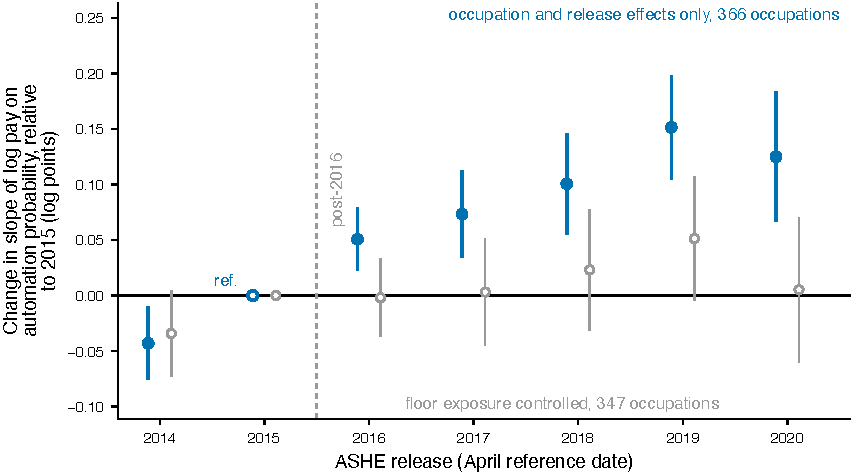
\includegraphics[width=0.94\textwidth]{fig2_pay_event_floor.pdf}
\caption{Event-study estimates for log mean hourly pay relative to 2015, with and without exposure to the wage floor. Each point is $\hat{\beta}_s$ from equation~\eqref{eq:es}, the change between 2015 and release $s$ in the cross-occupation slope of log mean gross hourly pay on the ONS automation probability, with 95 per cent intervals from standard errors clustered by occupation. The accent series conditions on occupation and release effects only, and its 2014 point sits below zero by as much as its 2016 point sits above it, so the gradient was compressing before the treatment date at the rate it compressed after. The grey series adds the interaction between the 2015 share of the occupation's jobs paid below \pounds 7.20 and each release indicator, and every post-2016 point then lies within its interval of zero. \emph{Source:} ASHE Table 14.5a, 2014--2020 releases; ONS (2019).}
\label{fig:espay}
\end{figure}

Table~\ref{tab:trend} states the same finding in one parameter. On the 2014 to 2019 releases the gradient trends at 0.037 (0.006) per year when no break is allowed. When a 2016 break is added the trend is 0.034 (0.007) and the break 0.015 (0.020), with a confidence interval of $[-0.025, 0.054]$. On the 2014 to 2020 releases the trend is 0.024 (0.007) and the break 0.039 (0.021), with an interval that includes zero. With the median as the outcome the trend is 0.027 (0.006) and the break 0.044 (0.020). RQ1 is answered fully. The pay gradient became less negative after 2016. The movement continues a compression already under way between the 2014 and 2015 releases at a steady pace to 2019, with no break at the treatment date that the data can distinguish from zero.

\begin{table}[!ht]\centering
\caption{Linear trend or break at 2016 in the automation-risk gradient}\label{tab:trend}
\begin{threeparttable}\footnotesize\setlength{\tabcolsep}{3pt}
\begin{tabular}{lcccccc}\toprule
 & (1) & (2) & (3) & (4) & (5) & (6) \\
Dependent variable & Pay & Pay & Pay & Pay & Jobs & Jobs \\
Releases & 2014--19 & 2014--19 & 2014--20 & 2014--20 & 2014--19 & 2014--20 \\ \midrule
Risk $\times$ (year $-$ 2015) & 0.037 & 0.034 & 0.031 & 0.024 & -0.083 & -0.146 \\
 & (0.006) & (0.007) & (0.005) & (0.007) & (0.021) & (0.018) \\
Risk $\times$ post-2016 & -- & 0.015 & -- & 0.039 & -0.120 & 0.036 \\
 &  & (0.020) &  & (0.021) & (0.059) & (0.063) \\ \addlinespace
Occupation-years & 2,184 & 2,184 & 2,546 & 2,546 & 1,842 & 2,149 \\
Occupations & 366 & 366 & 366 & 366 & 307 & 307 \\
\bottomrule\end{tabular}
\begin{tablenotes}\footnotesize
\item \emph{Notes:} Estimates of equation (3). The trend term lets the risk gradient move linearly in calendar time and the break term adds a level shift from 2016. Pay is log mean gross hourly pay on the full panel; jobs is log employee jobs on the balanced panel of 309 occupations with a published count in every release. All columns include occupation and release fixed effects. Standard errors clustered by occupation are reported in parentheses.
\item \emph{Source:} ASHE Table 14, 2014--2020 releases, revised editions; ONS (2019) probability of automation.
\end{tablenotes}\end{threeparttable}\end{table}

\subsection{The Wage Floor}

Table~\ref{tab:nlw} reports equation~\eqref{eq:nlw} on the 347 occupations for which the floor-exposure share can be computed. Column 1 restates the pay interaction on this sample at 0.132 (0.018). Column 2 adds the interaction between the 2015 share of jobs below \pounds 7.20 and the post-2016 indicator. The risk coefficient falls to 0.033 (0.021), with an interval of $[-0.008, 0.074]$, while the floor coefficient is 0.164 (0.017). An occupation with a tenth more of its jobs below the incoming floor grew 1.6 log points faster after 2016, and once that is allowed for the probability adds nothing that the data can distinguish from zero. Column 3 adds the triple interaction, which is $-0.108$ (0.197) and uninformative. Columns 4 and 5 replace the share with the Kaitz index, and the risk coefficient becomes $-0.047$ (0.031) and $-0.025$ (0.033), with the Kaitz interaction at 0.154 (0.026). The two exposure measures agree that the post-2016 pay movement belongs to the floor. Appendix~\ref{app:theory} works out what magnitude the floor coefficient should take under the framework and finds the estimate above the implied lower bound.

\begin{table}[!ht]\centering
\caption{The post-2016 pay gradient conditional on exposure to the National Living Wage}\label{tab:nlw}
\begin{threeparttable}\footnotesize\setlength{\tabcolsep}{4pt}
\begin{tabular}{lccccc}\toprule
 & (1) & (2) & (3) & (4) & (5) \\
Exposure measure & None & Share below floor & Share below floor & Kaitz index & Kaitz index \\ \midrule
Risk $\times$ post & 0.132 & 0.033 & 0.025 & -0.047 & -0.025 \\
 & (0.018) & (0.021) & (0.026) & (0.031) & (0.033) \\
Exposure $\times$ post &  & 0.164 & 0.233 & 0.154 & -0.008 \\
 &  & (0.017) & (0.133) & (0.026) & (0.065) \\
Risk $\times$ exposure $\times$ post &  &  & -0.108 &  & 0.326 \\
 &  &  & (0.197) &  & (0.103) \\ \addlinespace
Occupation-years & 2,426 & 2,426 & 2,426 & 2,426 & 2,426 \\
Occupations & 347 & 347 & 347 & 347 & 347 \\
\bottomrule\end{tabular}
\begin{tablenotes}\footnotesize
\item \emph{Notes:} Estimates of equation (4) on the 347 occupations for which the 2015 percentiles allow the exposure share to be computed. The dependent variable is log mean gross hourly pay. The share below the floor is the interpolated share of the occupation's employee jobs paid below \pounds 7.20 in the 2015 release; the Kaitz index is \pounds 7.20 divided by the occupation's 2015 median hourly pay. Both are demeaned across occupations, so the coefficient on risk in columns 3 and 5 is evaluated at mean exposure. The exposure share correlates 0.60 and the Kaitz index 0.82 with the automation probability. All columns include occupation and release fixed effects. Standard errors clustered by occupation are reported in parentheses.
\item \emph{Source:} ASHE Table 14, 2014--2020 releases, revised editions; ONS (2019) probability of automation.
\end{tablenotes}\end{threeparttable}\end{table}

The event-study version removes the linear restriction. Column 3 of Table~\ref{tab:espay} interacts the share with every release indicator. The risk coefficients for 2016 to 2020 then become $-0.002$ (0.018), 0.003 (0.025), 0.023 (0.028), 0.051 (0.028) and 0.005 (0.033), against 0.051, 0.073, 0.101, 0.151 and 0.125 without the control. The 2014 coefficient moves from $-0.043$ to $-0.034$ (0.020), so the pre-period difference is partly the floor as well, which is consistent with the National Minimum Wage upratings of October 2014 and October 2015 that preceded the NLW. Appendix~\ref{app:extra} reports the earlier version's proxy, in which the occupation's 2014 log pay replaces the exposure share, and reaches the same reading with less precision. RQ2 is answered fully. Exposure to the wage floor accounts for the post-2016 movement in the pay gradient, and the automation probability carries no association with post-2016 pay growth beyond the one it shares with low pay.

\subsection{Employment and Hours}

Table~\ref{tab:jobs} reports equation~\eqref{eq:twfe} for log employee jobs and log hours. On the 346 occupations with any published jobs count the interaction is $-0.501$ (0.057), and on the 309 occupations with a count in every release it is $-0.483$ (0.057), with an interval of $[-0.594, -0.371]$. An occupation one standard deviation more automatable therefore had employment about 7.0 log points lower after 2016 relative to before, or 6.8 per cent, conditional on occupation and release effects. The estimate is $-0.374$ (0.055) on the 2014 to 2019 releases, which exclude the April 2020 reference date, and $-0.359$ (0.054) when weighted by 2015 jobs. Column 5 adds the floor-exposure interaction. The risk coefficient is $-0.536$ (0.072) with the floor coefficient at 0.099 (0.059), so exposure to the floor does not account for the employment loss, and the point estimate suggests that occupations more exposed to the floor lost slightly less. Hours in column 6 move little, at $-0.027$ (0.013).

\begin{table}[!ht]\centering
\caption{Post-2016 change in the automation-risk gradient of log employment and log hours}\label{tab:jobs}
\begin{threeparttable}\scriptsize\setlength{\tabcolsep}{2pt}
\begin{tabular}{lcccccc}\toprule
 & (1) & (2) & (3) & (4) & (5) & (6) \\
 & Jobs, all & Balanced & Bal., 2014--19 & Bal., weighted & Bal., floor & Hours \\ \midrule
Risk $\times$ post-2016 & -0.501 & -0.483 & -0.374 & -0.359 & -0.536 & -0.027 \\
 & (0.057) & (0.057) & (0.055) & (0.054) & (0.072) & (0.013) \\
95\% confidence interval & [-0.613, -0.388] & [-0.594, -0.371] & [-0.483, -0.266] & [-0.465, -0.252] & [-0.677, -0.396] & [-0.053, -0.001] \\
Floor share $\times$ post-2016 & & & & & 0.099 & \\
 & & & & & (0.059) & \\ \addlinespace
Occupation-years & 2,293 & 2,163 & 1,854 & 2,149 & 2,149 & 2,550 \\
Occupations & 346 & 309 & 309 & 307 & 307 & 367 \\
\bottomrule\end{tabular}
\begin{tablenotes}\footnotesize
\item \emph{Notes:} Estimates of equation (1) with log employee jobs (columns 1 to 5) or log mean paid hours per week (column 6) as the dependent variable. Columns 2 to 5 keep the 309 occupations with a published jobs count in all seven releases. Column 4 weights by 2015 jobs. Column 5 adds the interaction between the 2015 share of jobs below \pounds 7.20 and the post-2016 indicator. All columns include occupation and release fixed effects. Standard errors clustered by occupation are reported in parentheses.
\item \emph{Source:} ASHE Table 14, 2014--2020 releases, revised editions; ONS (2019) probability of automation.
\end{tablenotes}\end{threeparttable}\end{table}

Table~\ref{tab:esjobs} and Figure~\ref{fig:scissors} give the timing, and for employment the timing is a break. On the balanced panel the 2014 coefficient is $+0.095$ (0.044), so more automatable occupations were gaining employment relative to others between 2014 and 2015. The coefficients then run $-0.243$ (0.046), $-0.245$ (0.066), $-0.324$ (0.067), $-0.494$ (0.073) and $-0.869$ (0.083) from 2016 to 2020. The 2015-to-2016 increment of $-0.243$ is three times the size of any increment before 2019, and it reverses the sign of the pre-period movement. Column 2 shows the same sequence with the floor share interacted with every release, at $+0.078$, $-0.228$, $-0.300$, $-0.444$, $-0.613$ and $-0.902$. The hours coefficients in column 3 lie within their intervals of zero until 2019 and reach $-0.094$ (0.023) only in 2020. Columns 5 and 6 of Table~\ref{tab:trend} fit the trend-and-break model to employment. On 2014 to 2019 both terms carry weight, at $-0.083$ (0.021) for the trend and $-0.120$ (0.059) for the break, whereas the 2020 release pushes the fit towards the trend because the pandemic reference date drives the largest drop.

\begin{table}[!ht]\centering
\caption{Event-study estimates for log employment and log hours, relative to 2015}\label{tab:esjobs}
\begin{threeparttable}\footnotesize\setlength{\tabcolsep}{4pt}
\begin{tabular}{lcccccc}\toprule
 & \multicolumn{2}{c}{(1) Jobs, balanced} & \multicolumn{2}{c}{(2) Jobs, floor controlled} & \multicolumn{2}{c}{(3) Hours} \\
\cmidrule(lr){2-3}\cmidrule(lr){4-5}\cmidrule(lr){6-7}
Release & $\hat{\beta}_{s}$ & (s.e.) & $\hat{\beta}_{s}$ & (s.e.) & $\hat{\beta}_{s}$ & (s.e.) \\ \midrule
2014 & 0.095 & (0.044) & 0.078 & (0.046) & 0.017 & (0.012) \\
2015 & 0 (ref.) &  & 0 (ref.) &  & 0 (ref.) &  \\
2016 & -0.243 & (0.046) & -0.228 & (0.055) & -0.002 & (0.016) \\
2017 & -0.245 & (0.066) & -0.300 & (0.076) & 0.024 & (0.021) \\
2018 & -0.324 & (0.067) & -0.444 & (0.086) & 0.011 & (0.016) \\
2019 & -0.494 & (0.073) & -0.613 & (0.090) & -0.031 & (0.018) \\
2020 & -0.869 & (0.083) & -0.902 & (0.111) & -0.094 & (0.023) \\
\addlinespace
Occupation-years & \multicolumn{2}{c}{2,163} & \multicolumn{2}{c}{2,149} & \multicolumn{2}{c}{2,550} \\
Occupations & \multicolumn{2}{c}{309} & \multicolumn{2}{c}{307} & \multicolumn{2}{c}{367} \\
\bottomrule\end{tabular}
\begin{tablenotes}\footnotesize
\item \emph{Notes:} Estimates of $\beta_{s}$ in equation (2) with the stated dependent variable and 2015 omitted. Column 2 adds the interaction between the 2015 floor-exposure share and each release indicator. A negative coefficient means employment in more automatable occupations was lower in that release, relative to 2015, than in less automatable ones. All columns include occupation and release fixed effects. Standard errors clustered by occupation are reported in parentheses.
\item \emph{Source:} ASHE Table 14, 2014--2020 releases, revised editions; ONS (2019) probability of automation.
\end{tablenotes}\end{threeparttable}\end{table}

\begin{figure}[!ht]
\centering
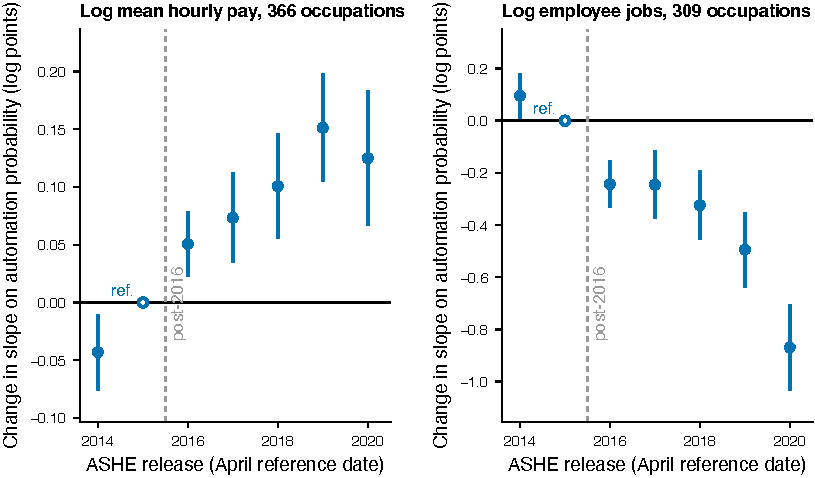
\includegraphics[width=0.94\textwidth]{fig3_pay_jobs_scissors.pdf}
\caption{Pay and employment moved in opposite directions across the automation-risk gradient. Each point is $\hat{\beta}_s$ from equation~\eqref{eq:es}, the change between 2015 and release $s$ in the cross-occupation slope of the stated outcome on the ONS automation probability, with 95 per cent intervals from standard errors clustered by occupation. The left panel covers log mean gross hourly pay for 366 occupations and the right panel log employee jobs for the 309 occupations with a published count in every release. The two panels share a unit and carry different scales, since the employment coefficients are four to seven times the pay coefficients. The pay gradient rises along a path that passes through the pre-period, whereas the employment gradient is above zero in 2014 and falls from 2016 onward. \emph{Source:} ASHE Table 14.5a, 2014--2020 releases; ONS (2019).}
\label{fig:scissors}
\end{figure}

The raw counts behind the estimates tell the same story without a regression. Among the 309 balanced occupations, total employee jobs rose from 24.7 million in 2014 to 26.5 million in 2019, while the share in above-median-risk occupations fell from 54.1 per cent in 2015 to 50.8 in 2019 and 48.0 in 2020. Employment in the lowest-risk tercile grew by 10.2 log points between 2015 and 2019, in the middle tercile by 1.6, and in the highest-risk tercile it fell by 3.2. Across the 324 occupations with both series in 2015 and 2019, the change in log employment correlates $-0.37$ with the probability while the change in log mean pay correlates $+0.36$, and the two changes correlate $-0.06$ with each other. RQ3 is answered in full for employment and negatively for hours. Employment in more automatable occupations fell relative to others from 2016 onward, after a pre-period in which it had been rising, and the fall is not explained by exposure to the wage floor. Hours moved little until 2020.

The three answers fit one account, which Appendix~\ref{app:theory} sets out. A shift in labour demand against automatable tasks lowers employment in the occupations that hold them, and lowers their wage index where the wage is free to fall. A statutory floor that binds for a share $F_i$ of the occupation's jobs prevents the fall for those jobs and raises the observed mean by $F_i$ per unit increase in the floor, as Proposition~\ref{prop:floor} shows. The exit of jobs paid below the occupation's mean raises the mean of those who remain, as Proposition~\ref{prop:composition} shows. An exposure-score regression on mean pay alone therefore records a positive interaction from the floor and from composition, and reads a labour market in which the exposed occupations were losing employment as one in which they were gaining. The employment margin is where the probability predicts what the task-based tradition expects.

\section{Alternative Specifications}\label{sec:sens}

Table~\ref{tab:rob} collects the alternative specifications for pay. Replacing the continuous probability with an above-median indicator gives 0.032 (0.006), and terciles give 0.010 (0.007) for the middle third and 0.036 (0.007) for the top third relative to the bottom, so the movement is monotone in the dose. Replacing release fixed effects with major-group-by-release effects, which allow each of the nine one-digit SOC groups its own pay path, gives 0.186 (0.066). Sub-major-group-by-release effects across 25 two-digit groups give 0.227 (0.084). Within a skill group the more automatable occupations are also the lower paid, so these estimates are the within-group counterpart of the same floor-driven compression.

\begin{table}[!ht]\centering
\caption{Alternative treatment definitions, time controls and cut-offs for log hourly pay}\label{tab:rob}
\begin{threeparttable}\footnotesize\setlength{\tabcolsep}{4pt}
\begin{tabular}{lccc}\toprule
Specification & Estimate & (s.e.) & 95\% confidence interval \\ \midrule
\multicolumn{4}{l}{\emph{Panel A. Discrete treatment}} \\
Above-median risk $\times$ post-2016 & 0.032 & (0.006) & [0.021, 0.043] \\
Middle risk tercile $\times$ post-2016 & 0.010 & (0.007) & [-0.003, 0.024] \\
Top risk tercile $\times$ post-2016 & 0.036 & (0.007) & [0.022, 0.049] \\
\addlinespace
\multicolumn{4}{l}{\emph{Panel B. Finer time controls}} \\
Risk $\times$ post-2016, major group $\times$ release effects & 0.186 & (0.066) & [0.055, 0.316] \\
Risk $\times$ post-2016, sub-major group $\times$ release effects & 0.227 & (0.084) & [0.062, 0.392] \\
\addlinespace
\multicolumn{4}{l}{\emph{Panel C. Alternative and placebo cut-offs}} \\
Risk $\times$ post-2017 & 0.110 & (0.018) & [0.075, 0.145] \\
Risk $\times$ post-2018 & 0.105 & (0.019) & [0.067, 0.143] \\
Risk $\times$ post-2019 & 0.102 & (0.020) & [0.062, 0.141] \\
Risk $\times$ post-2020 & 0.070 & (0.024) & [0.022, 0.117] \\
\addlinespace
Risk $\times$ post-2017, 2014--2019 releases only & 0.106 & (0.017) & [0.073, 0.140] \\
Risk $\times$ post-2018, 2014--2019 releases only & 0.106 & (0.019) & [0.069, 0.143] \\
\bottomrule\end{tabular}
\begin{tablenotes}\footnotesize
\item \emph{Notes:} Each row is a separate regression of log mean gross hourly pay on the stated interaction, estimated on the panel of 2,546 occupation-years unless the row restricts the releases. All columns include occupation and release fixed effects. unless the row names a finer time control. Risk terciles use cuts at 0.362 and 0.547 with the bottom tercile as the reference. Major groups are the nine one-digit SOC 2010 groups and sub-major groups the 25 two-digit groups. Standard errors clustered by occupation are reported in parentheses.
A permutation test that reassigns the automation probabilities at random across the 366 occupations 2,000 times, holding the panel fixed, produces a largest placebo interaction of 0.072 in absolute value, against the estimate of 0.122 in Table~\ref{tab:pay}, with a permutation standard deviation of 0.020.
\item \emph{Source:} ASHE Table 14, 2014--2020 releases, revised editions; ONS (2019) probability of automation.
\end{tablenotes}\end{threeparttable}\end{table}

Alternative cut-offs behave as a trend implies. Moving the treatment date to 2017, 2018, 2019 and 2020 gives 0.110, 0.105, 0.102 and 0.070 log points. On the 2014 to 2019 releases alone, placebo cut-offs at 2017 and 2018 return 0.106 (0.017) and 0.106 (0.019), the same as the 2016 estimate of 0.116 on those releases. A design in which every cut-off performs alike is measuring a trend. The permutation test reassigns the probabilities at random across occupations 2,000 times. The largest placebo interaction is 0.072 in absolute value against the estimate of 0.122 and the permutation standard deviation is 0.020, so the association between the probability and pay dynamics is not an artefact of the panel structure. Appendix~\ref{app:extra} reports the checks by level of 2014 pay from the earlier version, in which the pay interaction falls to $-0.015$ (0.037) once post-2016 growth varies with 2014 pay and to $-0.017$ (0.032) among occupations whose 2015 mean pay was \pounds 12 or more.

\section{The Classification Join}\label{sec:soc}

ASHE moved from SOC 2010 to SOC 2020 with the 2021 release, and the ONS dataset page for Table 14 on the SOC 2010 basis continues to host the later releases, so the workbook titles are the only warning. The workbooks inside the 2014 to 2020 zip archives are titled for SOC 2010 and those inside the 2021 to 2023 archives for SOC 2020. The 2021 release publishes a mean for 406 of 412 SOC 2020 unit groups. The earlier version of this paper joined the 2021 to 2023 releases to the SOC 2010 risk scores by numeric code, which kept the 261 codes that exist in both classifications. Of those 261 codes, 136 carry the same occupation title under both classifications and 125 carry a different one, so roughly half the post-2020 rows attached a 2017 risk score to a different occupation. Table~\ref{tab:soc} lists examples, among them code 1161, which denotes managers in transport and distribution under SOC 2010 and officers in the armed forces under SOC 2020.

The join manufactured the largest estimates in the earlier version. Table~\ref{tab:contam} and Figure~\ref{fig:contam} reproduce its design. With the mismatched releases included, the static pay interaction is 0.224 (0.030) against 0.122 (0.019) on the single-classification panel. The event-study coefficients for 2021, 2022 and 2023 are 0.425, 0.495 and 0.521, against a maximum of 0.151 on the clean panel. The earlier version read the post-2020 rise as the compression accelerating. It was the risk score being assigned to occupations it does not describe. Extending the panel past 2020 requires a crosswalk that allocates each SOC 2020 unit group to its SOC 2010 predecessors with employment weights, and this paper does not attempt it. The warning transfers. Any occupation-level exposure score is keyed to one classification, and any national series that changes classification mid-sample will match a large share of codes by number while matching a smaller share by meaning.

\section{Discussion and Conclusion}\label{sec:discussion}

The paper set out to test whether UK occupations the ONS rated more automatable lost employment or pay after 2016. They lost employment. Log employee jobs in an occupation one standard deviation more automatable fell by about 7 log points relative to others after 2016, with a break at the treatment date, a pre-period movement of the opposite sign, and no change once exposure to the wage floor is held fixed. Their mean pay rose relative to others by about 1.8 per cent per standard deviation, along a path that began between 2014 and 2015, moved linearly to 2019, and is accounted for by the share of the occupation's jobs paid below the incoming floor. The account in Appendix~\ref{app:theory} reconciles the two margins. Demand shifted against automatable tasks, the floor held pay up where it bound and raised observed means in proportion to exposure, and the exit of low-paid jobs raised the mean of those who remained. The earlier version read the pay interaction as augmentation. That reading is not supported. The evidence is consistent with displacement on the quantity margin, and it is silent on augmentation because the design has no measure of what the remaining workers produce.

The limitations follow in decreasing order of consequence. First, the design has no measure of technology adoption and no date at which adoption began, so the paper cannot estimate a causal effect of AI on either margin. It can establish that the probability predicts relative employment loss with a break at 2016 and no pre-trend of the same sign, and that it predicts relative pay growth only through the level of pay. Second, the employment outcome is the published count of employee jobs from a 1 per cent sample with small counts suppressed, so the balanced employment panel covers 309 of 366 occupations and the excluded occupations are small. The unweighted, weighted and unbalanced estimates agree in sign and magnitude, which limits the concern without removing it. Third, the 2020 release has an April reference date that falls in the first pandemic lockdown, when large numbers of employees were furloughed and hours fell sharply. The 2020 coefficients for employment and hours therefore carry a shock unrelated to automation, and the 2014 to 2019 estimates carry the paper's conclusions on timing. Fourth, the floor-exposure share is interpolated from published percentiles and assumes a piecewise-linear pay distribution within an occupation; the Kaitz index, which needs no interpolation, gives the same reading. Fifth, each occupation receives equal weight in the main estimates, so they describe the average occupation, whereas the employment-weighted estimates describe the average worker and are larger for pay and smaller for employment. Sixth, the probability is a 2017 measure that predates large language models. \citet{arntz2017revisiting} show that occupation-level probabilities overstate task-level risk, so the measure is a noisy proxy for exposure to the technology now diffusing. None of these limitations affects the finding that the pay gradient was moving before 2016 at the rate it moved after, which rests on the two pre-treatment releases alone, or the finding that employment moved the other way.

Three extensions follow. A crosswalk from SOC 2020 to SOC 2010 with employment weights would carry the panel to 2023 and beyond on a consistent basis. The ASHE microdata, available through the Secure Research Service, would replace occupation means with individual pay histories and separate incumbent pay growth from composition directly, which is the decomposition of Proposition~\ref{prop:composition} taken to the data. The design also transfers to newer exposure measures. The AI Occupational Exposure index of \citet{felten2021occupational} and the language-model exposure of \citet{eloundou2024gpts} both rise with pay, so conditioning on the floor is the first check any UK application of them should run, and the employment margin is where the check should look first.

The result that survives is stated at its strength. Over 2014 to 2020, UK occupations rated most automatable in 2017 lost employment relative to the rest from 2016 onward and gained relative pay along a path that the wage floor explains. A single post-period regression on pay would have reported the opposite of what the employment series shows. The two series read together, with the floor held fixed, are consistent with the task-based tradition's prediction on the margin where wages could not adjust.

\begin{thebibliography}{99}
\setlength{\itemsep}{4pt}

\bibitem[Acemoglu and Restrepo(2019)]{acemoglu2019automation}
Acemoglu, Daron, and Pascual Restrepo. 2019. ``Automation and New Tasks: How Technology Displaces and Reinstates Labor.'' \emph{Journal of Economic Perspectives} 33 (2): 3--30.

\bibitem[Acemoglu and Restrepo(2020)]{acemoglu2020robots}
Acemoglu, Daron, and Pascual Restrepo. 2020. ``Robots and Jobs: Evidence from US Labor Markets.'' \emph{Journal of Political Economy} 128 (6): 2188--2244.

\bibitem[Acemoglu and Restrepo(2022)]{acemoglu2022tasks}
Acemoglu, Daron, and Pascual Restrepo. 2022. ``Tasks, Automation, and the Rise in US Wage Inequality.'' \emph{Econometrica} 90 (5): 1973--2016.

\bibitem[Acemoglu et al.(2022)]{acemoglu2022vacancies}
Acemoglu, Daron, David Autor, Jonathon Hazell, and Pascual Restrepo. 2022. ``Artificial Intelligence and Jobs: Evidence from Online Vacancies.'' \emph{Journal of Labor Economics} 40 (S1): S293--S340.

\bibitem[Arntz et al.(2017)]{arntz2017revisiting}
Arntz, Melanie, Terry Gregory, and Ulrich Zierahn. 2017. ``Revisiting the Risk of Automation.'' \emph{Economics Letters} 159: 157--160.

\bibitem[Autor et al.(2003)]{autor2003skill}
Autor, David H., Frank Levy, and Richard J. Murnane. 2003. ``The Skill Content of Recent Technological Change: An Empirical Exploration.'' \emph{Quarterly Journal of Economics} 118 (4): 1279--1333.

\bibitem[Autor et al.(2023)]{autor2023compression}
Autor, David, Arindrajit Dube, and Annie McGrew. 2023. ``The Unexpected Compression: Competition at Work in the Low Wage Labor Market.'' NBER Working Paper 31010, National Bureau of Economic Research, Cambridge, MA.

\bibitem[Brynjolfsson et al.(2025)]{brynjolfsson2025generative}
Brynjolfsson, Erik, Danielle Li, and Lindsey Raymond. 2025. ``Generative AI at Work.'' \emph{Quarterly Journal of Economics} 140 (2): 889--942.

\bibitem[Callaway et al.(2024)]{callaway2024continuous}
Callaway, Brantly, Andrew Goodman-Bacon, and Pedro H. C. Sant'Anna. 2024. ``Difference-in-Differences with a Continuous Treatment.'' NBER Working Paper 32117, National Bureau of Economic Research, Cambridge, MA.

\bibitem[Eloundou et al.(2024)]{eloundou2024gpts}
Eloundou, Tyna, Sam Manning, Pamela Mishkin, and Daniel Rock. 2024. ``GPTs Are GPTs: Labor Market Impact Potential of LLMs.'' \emph{Science} 384 (6702): 1306--1308.

\bibitem[Felten et al.(2021)]{felten2021occupational}
Felten, Edward, Manav Raj, and Robert Seamans. 2021. ``Occupational, Industry, and Geographic Exposure to Artificial Intelligence: A Novel Dataset and Its Potential Uses.'' \emph{Strategic Management Journal} 42 (12): 2195--2217.

\bibitem[Frey and Osborne(2017)]{frey2017future}
Frey, Carl Benedikt, and Michael A. Osborne. 2017. ``The Future of Employment: How Susceptible Are Jobs to Computerisation?'' \emph{Technological Forecasting and Social Change} 114: 254--280.

\bibitem[Giupponi et al.(2024)]{giupponi2024minimum}
Giupponi, Giulia, Robert Joyce, Attila Lindner, Tom Waters, Thomas Wernham, and Xiaowei Xu. 2024. ``The Employment and Distributional Impacts of Nationwide Minimum Wage Changes.'' \emph{Journal of Labor Economics} 42 (S1): S293--S333.

\bibitem[Graetz and Michaels(2018)]{graetz2018robots}
Graetz, Georg, and Guy Michaels. 2018. ``Robots at Work.'' \emph{Review of Economics and Statistics} 100 (5): 753--768.

\bibitem[Office for National Statistics(2019)]{ons2019automation}
Office for National Statistics. 2019. ``Which Occupations Are at Highest Risk of Being Automated?'' Article released 25 March. Office for National Statistics, Newport.

\bibitem[Office for National Statistics(2024)]{ons2024ashe}
Office for National Statistics. 2024. ``Earnings and Hours Worked, Occupation by Four-Digit SOC (2010): ASHE Table 14.'' Dataset, annual releases 2014 to 2023. Office for National Statistics, Newport.

\bibitem[Roth et al.(2023)]{roth2023trending}
Roth, Jonathan, Pedro H. C. Sant'Anna, Alyssa Bilinski, and John Poe. 2023. ``What's Trending in Difference-in-Differences? A Synthesis of the Recent Econometrics Literature.'' \emph{Journal of Econometrics} 235 (2): 2218--2244.

\bibitem[Webb(2020)]{webb2020impact}
Webb, Michael. 2020. ``The Impact of Artificial Intelligence on the Labor Market.'' Working Paper, Stanford University, Stanford, CA.

\end{thebibliography}

\clearpage
\appendix
\renewcommand{\thesection}{\Alph{section}}
\numberwithin{equation}{section}
\renewcommand{\theequation}{\thesection\arabic{equation}}
\numberwithin{table}{section}
\renewcommand{\thetable}{\thesection\arabic{table}}
\numberwithin{figure}{section}
\renewcommand{\thefigure}{\thesection\arabic{figure}}

\section{Framework and Derivations}\label{app:theory}

This appendix supports Sections~\ref{sec:strategy} and~\ref{sec:results}. Section~\ref{sec:results} reports that employment in more automatable occupations fell after 2016 while their mean pay rose, and that the pay movement is accounted for by exposure to the wage floor. Those two facts look contradictory if pay is read as the price of labour in the occupation. The purpose of this appendix is to show that they are not, by writing down the smallest model in which both occur together, and then to establish the four estimator properties the main text relies on. Every step is carried out in full so that a reader can check the algebra without reconstructing it.

\subsection{The Environment}

Consider occupation $i$ observed in release $t$. The occupation contains a continuum of employee jobs indexed by $j$. Pay in job $j$ is the product of an occupation-level wage index and a job-specific component,
\begin{equation}
w_{ijt} = \omega_{it}\,\epsilon_j ,
\end{equation}
where $\omega_{it} > 0$ is the wage index and $\epsilon_j > 0$ is drawn from a distribution with cumulative distribution function $G_i$ and density $g_i$, fixed over time within the occupation. The multiplicative form is what lets a single index summarise the occupation's price of labour while leaving the shape of its internal pay distribution free.

Labour demand for the occupation is
\begin{equation}
N^{d}_{it} = D_i\!\left(\omega_{it};\, z_{it}\right), \qquad z_{it} \equiv \tau_t A_i ,
\end{equation}
where $\tau_t \geq 0$ indexes the state of automation technology available in release $t$ and $A_i \in [0,1]$ is the share of the occupation's tasks that the technology can perform, which is the object the ONS probability measures. Demand is decreasing in the wage index and in the automation term,
\begin{equation}
\frac{\partial D_i}{\partial \omega} < 0, \qquad \frac{\partial D_i}{\partial z} < 0 .
\end{equation}
Labour supply to the occupation is
\begin{equation}
N^{s}_{it} = S_i\!\left(\omega_{it}\right), \qquad S_i' > 0 .
\end{equation}
A statutory floor $\bar{w}_t$ applies to every job, so pay as observed in the published statistics is
\begin{equation}\label{eq:obs}
w^{\mathrm{obs}}_{ijt} = \max\!\left(\omega_{it}\,\epsilon_j,\; \bar{w}_t\right).
\end{equation}
Equation~\eqref{eq:obs} is the only place the floor enters, and it is what separates the price of labour from the statistic the paper observes.

\subsection{Comparative Statics of an Automation Shock}

Suppose first that the floor does not bind anywhere in the occupation, so observed pay equals $\omega_{it}\epsilon_j$ throughout. Equilibrium requires
\begin{equation}
D_i\!\left(\omega_{it};\, z_{it}\right) = S_i\!\left(\omega_{it}\right).
\end{equation}
Totally differentiating with respect to $z$ and collecting terms in $d\omega$ gives
\begin{equation}
\frac{\partial D_i}{\partial \omega}\, d\omega + \frac{\partial D_i}{\partial z}\, dz = S_i'\, d\omega
\qquad \Longrightarrow \qquad
\frac{d\omega}{dz} = \frac{\partial D_i / \partial z}{S_i' - \partial D_i / \partial \omega} .
\end{equation}
The denominator is positive because $S_i' > 0$ and $\partial D_i / \partial \omega < 0$, and the numerator is negative, so $d\omega / dz < 0$. Employment follows from the supply curve,
\begin{equation}
\frac{dN_i}{dz} = S_i'\, \frac{d\omega}{dz} < 0 .
\end{equation}
Writing $\varepsilon^{S}_i$ for the elasticity of supply, $\varepsilon^{D}_i$ for the absolute elasticity of demand, and $\phi_i \equiv \partial \ln D_i / \partial z < 0$ for the proportional demand shift, the same two results in elasticity form are
\begin{equation}\label{eq:elast}
\frac{d \ln \omega_i}{dz} = \frac{\phi_i}{\varepsilon^{S}_i + \varepsilon^{D}_i},
\qquad
\frac{d \ln N_i}{dz} = \frac{\varepsilon^{S}_i\, \phi_i}{\varepsilon^{S}_i + \varepsilon^{D}_i} .
\end{equation}
Both are negative, and their ratio is the supply elasticity, $d \ln N_i / d \ln \omega_i = \varepsilon^{S}_i$. An automation shock with no floor therefore lowers pay and employment together, which is the prediction the pay margin of this paper fails to show.

Now suppose the floor binds at the margin, so the wage index cannot fall. Setting $d \ln \omega_i = 0$ in the demand curve leaves the whole adjustment on the quantity margin,
\begin{equation}\label{eq:bind}
\left.\frac{d \ln N_i}{dz}\right|_{\text{floor binds}} = \phi_i .
\end{equation}
Comparing \eqref{eq:bind} with \eqref{eq:elast} gives a sharp prediction, since $\varepsilon^{S}_i / (\varepsilon^{S}_i + \varepsilon^{D}_i) < 1$ implies
\begin{equation}
\left| \left.\frac{d \ln N_i}{dz}\right|_{\text{floor binds}} \right| \; > \; \left| \left.\frac{d \ln N_i}{dz}\right|_{\text{floor slack}} \right| .
\end{equation}
The employment loss from a given automation shock should be larger where the floor binds. Table~\ref{tab:jobs} column 5 tests this by interacting floor exposure with the post-2016 indicator in the employment regression. The coefficient is $0.099$ with a standard error of $0.059$ and an interval of $[-0.016, 0.215]$, so it is not distinguishable from zero, and its point estimate carries the opposite sign to the prediction. The prediction is recorded here as unsupported. Two features of the setting would attenuate or reverse it, namely that the floor also raises the cost of labour in exposed occupations relative to their own counterfactual, and that the exposure share is measured at a single date, but neither is tested in this paper.

\subsection{The Floor-Exposure Share as the First-Order Effect on Mean Pay}

The regression in equation~\eqref{eq:nlw} uses the share of an occupation's jobs paid below the incoming floor as the measure of exposure. This subsection derives that choice. Define the occupation's mean observed pay from \eqref{eq:obs}, holding the wage index and the distribution $G_i$ fixed,
\begin{equation}\label{eq:mdef}
m_{it} \;=\; \mathbb{E}\!\left[\max\!\left(\omega_{it}\epsilon,\; \bar{w}_t\right)\right]
\;=\; \int_{0}^{a_{it}} \bar{w}_t \, dG_i(\epsilon) \;+\; \int_{a_{it}}^{\infty} \omega_{it}\,\epsilon \, dG_i(\epsilon),
\qquad a_{it} \equiv \frac{\bar{w}_t}{\omega_{it}},
\end{equation}
and define the share of jobs paid at or below the floor,
\begin{equation}\label{eq:Fdef}
F_{it} \;=\; \Pr\!\left(\omega_{it}\epsilon \leq \bar{w}_t\right) \;=\; G_i\!\left(a_{it}\right).
\end{equation}

\begin{proposition}\label{prop:floor}
Holding the wage index $\omega_{it}$ and the distribution $G_i$ fixed, the derivative of mean observed pay with respect to the floor equals the share of jobs at or below the floor,
\begin{equation}
\frac{\partial m_{it}}{\partial \bar{w}_t} \;=\; F_{it}.
\end{equation}
\end{proposition}

\begin{proof}
Differentiate the two terms of \eqref{eq:mdef} in turn, noting that $\partial a_{it} / \partial \bar{w}_t = 1/\omega_{it}$. The first term is $\bar{w}_t\, G_i(a_{it})$, and by the product rule
\begin{equation}
\frac{\partial}{\partial \bar{w}_t}\left[\bar{w}_t\, G_i(a_{it})\right]
= G_i(a_{it}) + \bar{w}_t\, g_i(a_{it})\,\frac{1}{\omega_{it}} .
\end{equation}
The second term is $\omega_{it}\int_{a_{it}}^{\infty}\epsilon\, dG_i(\epsilon)$, and by the Leibniz rule, since the upper limit is fixed and the lower limit moves,
\begin{equation}
\frac{\partial}{\partial \bar{w}_t}\left[\omega_{it}\int_{a_{it}}^{\infty}\epsilon\, dG_i(\epsilon)\right]
= -\,\omega_{it}\, a_{it}\, g_i(a_{it})\,\frac{1}{\omega_{it}}
= -\,\bar{w}_t\, g_i(a_{it})\,\frac{1}{\omega_{it}},
\end{equation}
where the last equality substitutes $\omega_{it} a_{it} = \bar{w}_t$ from \eqref{eq:mdef}. The two density terms are equal in magnitude and opposite in sign, so they cancel, and adding the two derivatives leaves
\begin{equation}
\frac{\partial m_{it}}{\partial \bar{w}_t} = G_i(a_{it}) = F_{it},
\end{equation}
which is the claim. The cancellation is the statement that a job exactly at the floor is indifferent between the two branches of \eqref{eq:obs}, so moving it across the boundary changes nothing.
\end{proof}

Two consequences matter for the empirical work. First, differentiating once more,
\begin{equation}
\frac{\partial^{2} m_{it}}{\partial \bar{w}_t^{2}} = \frac{g_i(a_{it})}{\omega_{it}} \;\geq\; 0,
\end{equation}
so mean observed pay is convex in the floor. A discrete uprating from $\bar{w}_0$ to $\bar{w}_1$ therefore satisfies
\begin{equation}\label{eq:discrete}
m(\bar{w}_1) - m(\bar{w}_0) \;=\; \int_{\bar{w}_0}^{\bar{w}_1} F(t)\, dt \;\geq\; F(\bar{w}_0)\left(\bar{w}_1 - \bar{w}_0\right),
\end{equation}
because $F$ is increasing. Using the share measured before the uprating, as equation~\eqref{eq:nlw} does, understates the effect of a discrete rise. Second, the regression uses log mean pay, so the object the coefficient $\theta$ approximates is
\begin{equation}
\frac{\partial \ln m_{it}}{\partial F_{it}} \;\approx\; \frac{\bar{w}_1 - \bar{w}_0}{m_{it}},
\end{equation}
which varies across occupations with the level of mean pay. Evaluating it at $F_i = 1$, where the whole of the occupation's pay distribution lies below the incoming floor, gives a bound that needs no knowledge of $\omega_i$ or $G_i$.

\begin{proposition}\label{prop:bound}
For an occupation with $F_i = 1$ in the base release, the change in log mean observed pay between the base release and release $t$ is at least $\ln\!\left(\bar{w}_t / \bar{w}_{2016}\right)$.
\end{proposition}

\begin{proof}
If $F_i = 1$ then every job in the occupation is paid below $\bar{w}_{2016}$ in the base release, so $m_{i,2015} \leq \bar{w}_{2016}$. In release $t$ the floor applies to every job, so $m_{it} \geq \bar{w}_t$ by \eqref{eq:obs}. Taking logs of the ratio gives
\begin{equation}
\ln m_{it} - \ln m_{i,2015} \;\geq\; \ln \bar{w}_t - \ln \bar{w}_{2016},
\end{equation}
which is the claim.
\end{proof}

The NLW rates in April of 2016 to 2020 were \pounds 7.20, \pounds 7.50, \pounds 7.83, \pounds 8.21 and \pounds 8.72, so the implied per-release lower bounds are $0.000$, $0.041$, $0.084$, $0.131$ and $0.192$ log points, and their average over the five post-2016 releases is $0.090$. Since $\theta$ in equation~\eqref{eq:nlw} is the coefficient on a demeaned share and the post-2016 indicator pools those five releases, the estimate of $\theta$ extrapolated to $F_i = 1$ should be at least $0.090$, provided that occupations with no jobs below the floor experience no floor-driven growth of their own. The estimate in Table~\ref{tab:nlw} column 2 is $0.164$ with a standard error of $0.017$, which is above the bound. Because the third branch of equation~\eqref{eq:share} caps the share at the highest published rank, no occupation in the sample attains $F_i = 1$, and the comparison extrapolates the linear coefficient to that point. The excess is consistent with spillovers above the floor within exposed occupations, which \citet{giupponi2024minimum} document up to roughly the twentieth percentile over these years, and with the composition term of Proposition~\ref{prop:composition}. Spillovers that reached occupations with no jobs below the floor would work in the other direction, by raising the growth of the comparison group, so the bound serves as a benchmark only.

\subsection{Composition and the Occupational Mean}

The published statistic is the mean pay of whoever holds the occupation's jobs in that release, so a change in it mixes pay growth for continuing jobs with a change in which jobs exist. This subsection separates the two exactly. Let the occupation hold $N_{t-1}$ jobs in release $t-1$ with mean pay $m_{t-1}$. Let $E$ of those jobs disappear by release $t$, with mean pay $m^{L}_{t-1}$ measured at $t-1$, and let each of the $N_t = N_{t-1} - E$ surviving jobs change pay by $\Delta w_j$. Suppose for the moment that no new jobs enter.

\begin{proposition}\label{prop:composition}
The change in the occupation's mean pay decomposes as
\begin{equation}\label{eq:decomp}
m_t - m_{t-1} \;=\; \underbrace{\frac{1}{N_t}\sum_{j \in \mathrm{stayers}} \Delta w_j}_{\text{pay growth of continuing jobs}} \;+\; \underbrace{\frac{E}{N_t}\left(m_{t-1} - m^{L}_{t-1}\right)}_{\text{composition}} .
\end{equation}
\end{proposition}

\begin{proof}
The total wage bill in release $t$ is the bill at $t-1$, less the bill of the jobs that left, plus the pay changes of those that stayed,
\begin{equation}
N_t\, m_t \;=\; N_{t-1}\, m_{t-1} \;-\; E\, m^{L}_{t-1} \;+\; \sum_{j \in \mathrm{stayers}} \Delta w_j .
\end{equation}
Divide by $N_t$ and substitute $N_{t-1} = N_t + E$,
\begin{equation}
m_t \;=\; m_{t-1} + \frac{E}{N_t}\, m_{t-1} - \frac{E}{N_t}\, m^{L}_{t-1} + \frac{1}{N_t}\sum_{j \in \mathrm{stayers}} \Delta w_j ,
\end{equation}
and collecting the two terms in $E / N_t$ gives \eqref{eq:decomp}.
\end{proof}

The composition term is positive whenever the jobs that disappear paid less than the occupation's average, which is the case when a contraction is concentrated at the bottom of an occupation's pay distribution. A fall in employment can therefore raise measured mean pay with no worker receiving a rise. Allowing entry adds a symmetric term. If $B$ jobs enter at mean pay $m^{B}_{t}$, the decomposition gains $(B / N_t)(m^{B}_{t} - m_{t-1})$, which is negative when entrants are paid below the incumbent average.

Section~\ref{sec:results} reports that across 324 occupations the change in log employment from 2015 to 2019 correlates $-0.37$ with the automation probability while the change in log mean pay correlates $+0.36$, which is the pairing \eqref{eq:decomp} produces when exit is concentrated at the bottom. The published series give $m_t$, $m_{t-1}$, $N_t$ and $N_{t-1}$ but not $m^{L}_{t-1}$ or the individual $\Delta w_j$, so the two terms cannot be separated here. The ASHE microdata identify both and would close this gap.

\subsection{Properties of the Estimators}

The remaining propositions justify four statements made in Section~\ref{sec:strategy} about what the regressions recover.

\begin{proposition}\label{prop:deflator}
Adding any release-specific constant to the dependent variable leaves every coefficient on an interaction with a release indicator, or with a function of $t$, unchanged in equations~\eqref{eq:twfe}, \eqref{eq:es}, \eqref{eq:trend} and \eqref{eq:nlw}.
\end{proposition}

\begin{proof}
Let $P_t$ denote a price index and write real log pay as $\ln w_{it} - \ln P_t$. Substituting into equation~\eqref{eq:twfe} gives
\begin{equation}
\ln w_{it} - \ln P_t = \alpha_i + \lambda_t + \beta \left( A_i \times \mathbf{1}[t \geq 2016] \right) + \varepsilon_{it},
\end{equation}
which rearranges to
\begin{equation}
\ln w_{it} = \alpha_i + \left(\lambda_t + \ln P_t\right) + \beta \left( A_i \times \mathbf{1}[t \geq 2016] \right) + \varepsilon_{it}.
\end{equation}
The release effects are unrestricted, so $\lambda_t + \ln P_t$ is as admissible a set of release effects as $\lambda_t$, and the least-squares problem in $\beta$ is unchanged. The same substitution works for the other three equations because in each the deflator enters only through a term that depends on $t$ alone. Deflating therefore shifts the release effects and nothing else.
\end{proof}

\begin{proposition}\label{prop:static}
In equation~\eqref{eq:twfe} with a balanced panel of $T_0$ pre-treatment and $T_1$ post-treatment releases and equal weights, the static coefficient satisfies
\begin{equation}\label{eq:fwl}
\hat{\beta} = \frac{\mathrm{Cov}\!\left(\bar{y}^{\,\mathrm{post}}_i - \bar{y}^{\,\mathrm{pre}}_i,\; A_i\right)}{\mathrm{Var}\!\left(A_i\right)}
\end{equation}
and
\begin{equation}\label{eq:esavg}
\hat{\beta} = \frac{1}{T_1}\sum_{s \geq 2016} \hat{\beta}_s \;-\; \frac{1}{T_0}\sum_{s < 2016} \hat{\beta}_s ,
\end{equation}
where $\hat{\beta}_s$ are the event-study coefficients of equation~\eqref{eq:es} with any base release.
\end{proposition}

\begin{proof}
For \eqref{eq:fwl}, apply the Frisch--Waugh--Lovell theorem. Residualising the regressor $A_i P_t$ on occupation and release effects in a balanced panel gives $\left(A_i - \bar{A}\right)\left(P_t - \bar{P}\right)$, because $A_i$ is constant within an occupation and $P_t$ within a release. The least-squares coefficient of $y_{it}$ on that residual is
\begin{equation}
\hat{\beta} = \frac{\sum_i \sum_t \left(A_i - \bar{A}\right)\left(P_t - \bar{P}\right) y_{it}}{\sum_i \sum_t \left(A_i - \bar{A}\right)^{2}\left(P_t - \bar{P}\right)^{2}} .
\end{equation}
Summing over $t$ first, and using $\sum_t (P_t - \bar{P}) y_{it} = T_0 T_1 (\bar{y}^{\,\mathrm{post}}_i - \bar{y}^{\,\mathrm{pre}}_i) / (T_0 + T_1)$, the common factor cancels between numerator and denominator and leaves \eqref{eq:fwl}. For \eqref{eq:esavg}, note that equation~\eqref{eq:es} saturates the interaction of $A_i$ with the release indicators, so it fits the release-specific gradients exactly. The static regressor $A_i P_t$ is the projection of that saturated set onto $P_t$, and a projection onto a binary regressor with equal weights within each period returns the difference of the two period averages of the fitted gradients, which is \eqref{eq:esavg}.
\end{proof}

The paper's estimates satisfy \eqref{eq:esavg} numerically. For pay, the post-period average of the coefficients in Table~\ref{tab:espay} column 1 is $(0.051 + 0.073 + 0.101 + 0.151 + 0.125)/5 = 0.100$, the pre-period average with 2015 set to zero is $(-0.043 + 0)/2 = -0.021$, and the difference is $0.122$, which is the static estimate in Table~\ref{tab:pay} column 1. For employment on the balanced panel, the same calculation gives $-0.435 - 0.048 = -0.483$, which is the estimate in Table~\ref{tab:jobs} column 2 to three decimals. The pay identity holds to rounding because the pay panel is nearly balanced, with 2,546 of the $366 \times 7 = 2{,}562$ possible cells present, whereas the employment panel used here is balanced by construction.

\begin{proposition}\label{prop:restriction}
Equation~\eqref{eq:trend} is the restriction
\begin{equation}
\beta_s = \gamma\,(s - 2015) + \delta\, \mathbf{1}[s \geq 2016]
\end{equation}
imposed on the event-study coefficients of equation~\eqref{eq:es}.
\end{proposition}

\begin{proof}
Substitute the restriction into the summation in \eqref{eq:es} and collect terms,
\begin{equation}
\sum_{s \neq 2015} \beta_s \left(A_i \times \mathbf{1}[t=s]\right)
= \gamma \sum_{s \neq 2015} (s-2015) \left(A_i \times \mathbf{1}[t=s]\right) + \delta \sum_{s \geq 2016} \left(A_i \times \mathbf{1}[t=s]\right),
\end{equation}
and note that $\sum_{s}(s-2015)\mathbf{1}[t=s] = t - 2015$ and $\sum_{s \geq 2016}\mathbf{1}[t=s] = \mathbf{1}[t \geq 2016]$, which reproduces \eqref{eq:trend}.
\end{proof}

With one pre-treatment release the two parameters are identified from different features of the data. The trend $\gamma$ is identified from the slope across all seven releases, whereas the break $\delta$ is identified from the departure of the post-2016 coefficients from the line through the two pre-treatment points, so it rests on a single pre-period contrast. That is why the standard error on $\delta$ in Table~\ref{tab:trend} is about three times the standard error on $\gamma$, and why a paper with this pre-period can rule a break out only weakly while still establishing the trend.

\subsection{What the Static Coefficient Identifies}

\citet{callaway2024continuous} study exactly the design of equation~\eqref{eq:twfe} when the treatment is a continuous dose. Write $Y_{it}(a)$ for the outcome occupation $i$ would record in release $t$ under dose $a$, and define the average causal response at dose $a$ as the derivative of $\mathbb{E}[Y_{it}(a) - Y_{it}(0)]$ with respect to $a$. They show that the cross-sectional slope in \eqref{eq:fwl} equals a weighted average of that derivative only when the counterfactual change in the untreated outcome does not depend on the dose, which they call strong parallel trends,
\begin{equation}\label{eq:spt}
\mathbb{E}\!\left[\left. Y_{it}(0) - Y_{i,t-1}(0) \;\right|\; A_i = a \right] \; \text{does not vary with } a .
\end{equation}
When \eqref{eq:spt} fails, the slope in \eqref{eq:fwl} adds a selection term equal to the slope of the counterfactual change on the dose,
\begin{equation}
\hat{\beta} \;\xrightarrow{p}\; \underbrace{\text{weighted average causal response}}_{\text{the object of interest}} \;+\; \underbrace{\frac{\partial}{\partial a}\,\mathbb{E}\!\left[\left. Y_{it}(0) - Y_{i,t-1}(0) \;\right|\; A_i = a \right]}_{\text{selection on the counterfactual path}} .
\end{equation}
Condition \eqref{eq:spt} fails for pay in this setting by construction, since the dose correlates $-0.80$ with the 2014 level of pay and the level of pay determines exposure to a floor that rose throughout the post period. Equation~\eqref{eq:nlw} removes the part of the selection term that runs through floor exposure, which is why the risk coefficient there is the one the paper reads. It does not remove selection running through any other correlate of the dose, and the paper accordingly reports every static interaction as descriptive.

\section{Data Construction}\label{app:data}

This appendix supports Section~\ref{sec:data}. It records where each series comes from, how the panel is assembled, and how the floor-exposure share is computed, in enough detail for a reader to rebuild the panel from the public files.

\begin{table}[!ht]\centering
\caption{Workbook provenance and published cell counts, ASHE Table 14.5a}\label{tab:prov}
\begin{threeparttable}\footnotesize\setlength{\tabcolsep}{4pt}
\begin{tabular}{lccccc}\toprule
Release & Classification & Four-digit rows & Mean published & Median published & Jobs published \\ \midrule
2014 & SOC10 & 369 & 364 & 361 & 342 \\
2015 & SOC10 & 369 & 365 & 360 & 334 \\
2016 & SOC10 & 369 & 365 & 359 & 329 \\
2017 & SOC10 & 369 & 363 & 361 & 329 \\
2018 & SOC10 & 369 & 364 & 358 & 329 \\
2019 & SOC10 & 369 & 363 & 352 & 329 \\
2020 & SOC10 & 369 & 362 & 348 & 311 \\
2021 & SOC20 & 412 & 406 & 398 & 357 \\
2022 & SOC20 & 412 & 408 & 380 & 355 \\
2023 & SOC20 & 412 & 408 & 405 & 362 \\
\bottomrule\end{tabular}
\begin{tablenotes}\footnotesize
\item \emph{Notes:} Each release is the revised edition downloaded from the ONS dataset page for ASHE Table 14 on the SOC 2010 basis. Counts are four-digit unit-group rows on the All sheet of Table 14.5a carrying a value that is not suppressed in the stated column. The 2021 to 2023 workbooks are titled for SOC 2020 and enter the analysis only in Appendix D.
\item \emph{Source:} ASHE Table 14, 2014--2020 releases, revised editions; ONS (2019) probability of automation.
\end{tablenotes}\end{threeparttable}\end{table}

\subsection{Extraction}

For each release, the All sheet of Tables 14.5a, 14.6a and 14.9a is read and the header row located by the labels Description and Code. Rows whose code has exactly four digits are kept, which selects the unit groups and discards the major, sub-major and minor group rows that share the sheet. The columns read are the number of jobs in thousands, the median, the mean, and the ten published percentiles. The suppression markers used by the ONS, namely x, two dots, a colon and a dash, become missing, as does any cell that does not parse as a number. No release contains a duplicated four-digit code. The 2014 to 2020 releases contain 369 four-digit rows each, matching the 369 unit groups of SOC 2010, and the 2021 to 2023 releases contain 412, matching SOC 2020. The panel keeps the 2014 to 2020 releases and joins the ONS probability by four-digit code, which matches 366 occupations with at least one published mean. Rebuilding the archived panel of the earlier version from the raw files reproduces all 2,546 of its 2014 to 2020 cells to the last decimal, which fixes the reproducibility tier of every estimate in this paper as recomputed from raw data.

\subsection{The Floor-Exposure Share}

The share of an occupation's jobs paid below the incoming floor is not published, so it is interpolated from the percentiles that are. For occupation $i$ in the 2015 release, let $(q_k, p_k)$ for $k = 1, \dots, K$ denote the published percentile values and their ranks, including the median at rank 50, sorted in increasing order of value, with any suppressed percentile omitted. Treating the pay distribution as piecewise linear between adjacent published percentiles, the share of jobs paid below a threshold $\bar{w}$ is
\begin{equation}\label{eq:share}
F_i(\bar{w}) \;=\; \frac{1}{100}
\begin{cases}
\max\!\left\{0,\; p_1 - \dfrac{p_2 - p_1}{q_2 - q_1}\left(q_1 - \bar{w}\right)\right\}, & \bar{w} \leq q_1, \\[14pt]
p_k + \dfrac{p_{k+1} - p_k}{q_{k+1} - q_k}\left(\bar{w} - q_k\right), & q_k < \bar{w} \leq q_{k+1}, \\[14pt]
p_K, & \bar{w} > q_K .
\end{cases}
\end{equation}
The paper sets $\bar{w} = 7.20$, the NLW rate of April 2016. The middle branch is ordinary linear interpolation within the bracketing segment. The first branch extrapolates below the lowest published percentile using the slope of the lowest published segment and clamps the result at zero, so an occupation whose tenth percentile lies far above the floor receives a share of zero where the linear extrapolation would return a negative number. The third branch assigns the highest published rank when the threshold exceeds the ninetieth percentile. The share is computed only where at least three percentiles are published, which holds for 347 of the 366 occupations. The Kaitz index is $\bar{w} / q_{50}$ and needs no interpolation.

Two worked examples can be checked by hand against Table 14.5a of the 2015 release. Sales and retail assistants, code 7111, have a median of \pounds 7.11 at rank 50 and a sixtieth percentile of \pounds 7.41, so the threshold falls in the segment from rank 50 to rank 60 and the middle branch of \eqref{eq:share} gives
\begin{equation}
F_{7111} = \frac{1}{100}\left[50 + \frac{60 - 50}{7.41 - 7.11}\left(7.20 - 7.11\right)\right] = \frac{1}{100}\left[50 + 3.0\right] = 0.530 .
\end{equation}
Medical practitioners, code 2211, have a tenth percentile of \pounds 15.54 and a twentieth of \pounds 20.19, so the threshold lies below the lowest published percentile and the first branch applies,
\begin{equation}
F_{2211} = \frac{1}{100}\max\!\left\{0,\; 10 - \frac{20 - 10}{20.19 - 15.54}\left(15.54 - 7.20\right)\right\} = \frac{1}{100}\max\!\left\{0,\; -7.94\right\} = 0 .
\end{equation}
The two occupations sit at the extremes of the exposure distribution, which is what the correlation of $0.60$ between the share and the automation probability reflects.

\subsection{Weights and Samples}

Employment weights are the occupation's employee jobs in thousands in the 2015 release, published for 333 of the 366 pay occupations. The balanced pay panel keeps the 358 occupations with a published mean in every release from 2014 to 2020. The balanced employment panel keeps the 309 occupations with a published jobs count in every release. Table~\ref{tab:sample} reports the count of occupations with a published mean in each release, and Table~\ref{tab:prov} the counts for every column read.

\section{Additional Results}\label{app:extra}

This appendix supports Sections~\ref{sec:results} and~\ref{sec:sens}. Before the 2015 percentiles were used to build the floor-exposure share, the earlier version conditioned on the occupation's level of pay as a proxy for exposure. Table~\ref{tab:paylevel} reports those checks, which the share supersedes and with which it agrees.

\begin{table}[!ht]\centering
\caption{The post-2016 pay gradient by level of 2014 pay}\label{tab:paylevel}
\begin{threeparttable}\footnotesize\setlength{\tabcolsep}{4pt}
\begin{tabular}{lcccc}\toprule
Sample or specification & Risk $\times$ post & (s.e.) & Occ.-years & Occupations \\ \midrule
\multicolumn{5}{l}{\emph{Panel A. Conditioning on demeaned log 2014 pay, releases 2015--2020}} \\
Risk $\times$ post alone & 0.100 & (0.018) & 2,175 & 364 \\
Adding log 2014 pay $\times$ post & -0.015 & (0.037) & 2,175 & 364 \\
\quad coefficient on log 2014 pay $\times$ post & -0.054 & (0.018) & & \\
\addlinespace
\multicolumn{5}{l}{\emph{Panel B. Within terciles of 2014 mean hourly pay, releases 2015--2020}} \\
Bottom third of 2014 pay (\pounds6.74--11.17) & 0.104 & (0.042) & 725 & 121 \\
Middle third of 2014 pay (\pounds11.20--15.70) & 0.036 & (0.043) & 727 & 122 \\
Top third of 2014 pay (\pounds15.84--53.14) & 0.087 & (0.059) & 723 & 121 \\
\addlinespace
\multicolumn{5}{l}{\emph{Panel C. Dropping low-paid occupations, releases 2014--2020}} \\
2015 mean pay of \pounds8 or more & 0.101 & (0.019) & 2,466 & 354 \\
2015 mean pay of \pounds9 or more & 0.062 & (0.020) & 2,263 & 325 \\
2015 mean pay of \pounds10 or more & 0.040 & (0.021) & 2,046 & 294 \\
2015 mean pay of \pounds11 or more & 0.021 & (0.025) & 1,794 & 258 \\
2015 mean pay of \pounds12 or more & -0.017 & (0.032) & 1,542 & 222 \\
\bottomrule\end{tabular}
\begin{tablenotes}\footnotesize
\item \emph{Notes:} The dependent variable is log mean gross hourly pay. Panel A demeans the occupation's log mean pay in the 2014 release across occupations and excludes that release from estimation, so the conditioning variable is predetermined. The occupation-level correlation between the automation probability and log 2014 pay is -0.80. All columns include occupation and release fixed effects. Standard errors clustered by occupation are reported in parentheses.
\item \emph{Source:} ASHE Table 14, 2014--2020 releases, revised editions; ONS (2019) probability of automation.
\end{tablenotes}\end{threeparttable}\end{table}

Panel A demeans the occupation's log mean pay in the 2014 release, excludes that release from estimation so that the conditioning variable is predetermined, and interacts the demeaned level with the post-2016 indicator. The pay interaction falls from 0.100 (0.018) to $-0.015$ (0.037), with the coefficient on the pay level at $-0.054$ (0.018), so an occupation whose 2014 pay was one log point lower grew 5.4 log points faster after 2016. Panel B estimates the pay interaction within terciles of 2014 pay, at 0.104 (0.042) in the bottom third, 0.036 (0.043) in the middle and 0.087 (0.059) at the top. Panel C drops occupations whose 2015 mean pay lay below successive thresholds, and the interaction falls from 0.101 (0.019) above \pounds 8 to $-0.017$ (0.032) above \pounds 12, by which point the NLW rates of \pounds 7.20 to \pounds 8.72 no longer bind at the occupation's mean. The level of pay and the share below the floor therefore deliver the same reading, and the share is preferred because Proposition~\ref{prop:floor} gives it a structural interpretation that the level does not have.

\section{The Classification Join}\label{app:soc}

This appendix supports Section~\ref{sec:soc}. Table~\ref{tab:soc} lists the first six four-digit codes, in code order, that denote different occupations under SOC 2010 and SOC 2020 among the 261 codes that exist in both classifications. Table~\ref{tab:contam} and Figure~\ref{fig:contam} reproduce the earlier version's design with the mismatched releases included, so that the size of the resulting distortion can be read directly.

\begin{table}[!ht]\centering
\caption{Four-digit codes denoting different occupations under SOC 2010 and SOC 2020}\label{tab:soc}
\begin{threeparttable}\footnotesize\setlength{\tabcolsep}{4pt}
\begin{tabular}{lp{0.40\textwidth}p{0.40\textwidth}}\toprule
Code & SOC 2010 title, 2020 release & SOC 2020 title, 2021 release \\ \midrule
1132 & Marketing and sales directors & Marketing, sales and advertising directors \\
1133 & Purchasing managers and directors & Public relations and communications directors \\
1134 & Advertising and public relations directors & Purchasing managers and directors \\
1135 & Human resource managers and directors & Charitable organisation managers and directors \\
1136 & Information technology and telecommunications directors & Human resource managers and directors \\
1150 & Financial institution managers and directors & Managers and directors in retail and wholesale \\
\bottomrule\end{tabular}
\begin{tablenotes}\footnotesize
\item \emph{Notes:} The 2020 release publishes 369 four-digit SOC 2010 unit groups and the 2021 release 412 SOC 2020 unit groups. 261 numeric codes appear in both, of which 136 carry the same occupation title and 125 a different one. 151 SOC 2020 codes have no SOC 2010 counterpart and 108 SOC 2010 codes have no SOC 2020 counterpart. The rows are the first six mismatches in code order.
\item \emph{Source:} ASHE Table 14, 2014--2020 releases, revised editions; ONS (2019) probability of automation.
\end{tablenotes}\end{threeparttable}\end{table}
\begin{table}[!ht]\centering
\caption{Pay event study with and without the mismatched 2021--2023 releases}\label{tab:contam}
\begin{threeparttable}\footnotesize\setlength{\tabcolsep}{4pt}
\begin{tabular}{lcccc}\toprule
 & \multicolumn{2}{c}{SOC 2010 releases only} & \multicolumn{2}{c}{SOC 2020 releases joined by code} \\
\cmidrule(lr){2-3}\cmidrule(lr){4-5}
Release & $\hat{\beta}_{s}$ & (s.e.) & $\hat{\beta}_{s}$ & (s.e.) \\ \midrule
2014 & -0.043 & (0.017) & -0.043 & (0.017) \\
2015 & 0 (ref.) &  & 0 (ref.) &  \\
2016 & 0.051 & (0.014) & 0.050 & (0.014) \\
2017 & 0.073 & (0.020) & 0.072 & (0.020) \\
2018 & 0.101 & (0.023) & 0.100 & (0.023) \\
2019 & 0.151 & (0.024) & 0.151 & (0.024) \\
2020 & 0.125 & (0.030) & 0.128 & (0.030) \\
2021 & -- &  & 0.425 & (0.082) \\
2022 & -- &  & 0.495 & (0.081) \\
2023 & -- &  & 0.521 & (0.086) \\
\addlinespace
Risk $\times$ post-2016 & 0.122 & (0.019) & 0.224 & (0.030) \\
Occupation-years & \multicolumn{2}{c}{2,546} & \multicolumn{2}{c}{3,321} \\
\bottomrule\end{tabular}
\begin{tablenotes}\footnotesize
\item \emph{Notes:} The dependent variable is log mean gross hourly pay. The right-hand columns reproduce the design of the earlier version of this paper, in which the 2021 to 2023 releases, published on SOC 2020, were joined to SOC 2010 automation probabilities by numeric code. All columns include occupation and release fixed effects. Standard errors clustered by occupation are reported in parentheses.
\item \emph{Source:} ASHE Table 14, 2014--2020 releases, revised editions; ONS (2019) probability of automation.
\end{tablenotes}\end{threeparttable}\end{table}

\begin{figure}[!ht]
\centering
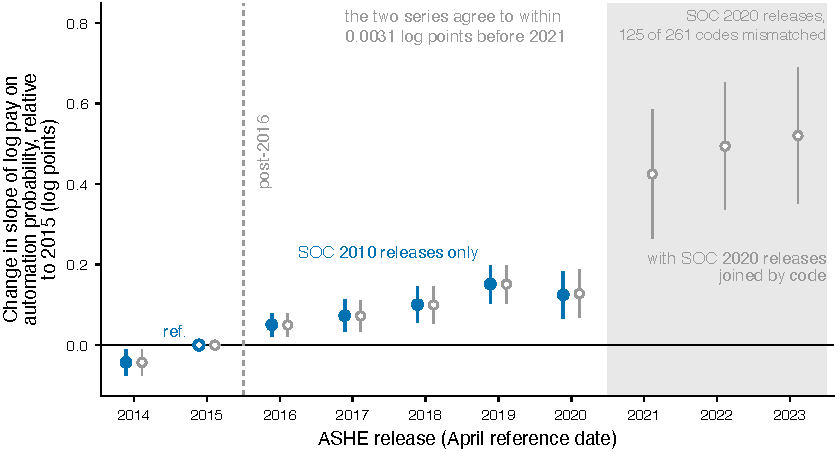
\includegraphics[width=0.94\textwidth]{figD1_classification_join.pdf}
\caption{The mismatched join manufactured the largest coefficients of the earlier version. Each point is $\hat{\beta}_s$ from equation~\eqref{eq:es} for log mean gross hourly pay relative to 2015, with 95 per cent intervals from standard errors clustered by occupation. The accent series uses the seven releases published on SOC 2010. The grey series adds the 2021 to 2023 releases, published on SOC 2020 and joined to SOC 2010 automation probabilities by numeric code, of which 125 of 261 denote a different occupation under the two classifications. The two series agree to within 0.0031 log points through 2020 and then diverge, the grey series reaching 0.52 log points where the probability is attached to occupations it does not describe. \emph{Source:} ASHE Table 14.5a, 2014--2023 releases; ONS (2019).}
\label{fig:contam}
\end{figure}

\section{Reproducibility and Withdrawn Claims}\label{app:repro}

This appendix supports Sections~\ref{sec:strategy} and~\ref{sec:soc}. Every estimate in this paper is recomputed from raw data. The panel is built from the public ASHE Table 14 workbooks by the archived script, the estimates are produced by the archived Python pipeline using the \texttt{pyfixest} package, every table is generated from a single locked file of estimates, and no number was transcribed by hand. The rebuilt panel reproduces the archived Stata panel of the earlier version for every 2014 to 2020 cell. The static pay interaction on those releases, 0.122 (0.019), reproduces the earlier version's own estimate on the same releases. The permutation test uses seed 20260912. No hypothesis was pre-registered, and the hypothesis of the earlier version was stated before its analysis and is recorded there.

Four claims from the earlier version are withdrawn and should not reappear. The outcome is not the median hourly wage, since the archived panel carries the mean; the median is now reported separately in Table~\ref{tab:pay}. Pay is not deflated to 2023 prices, since it is nominal, and Proposition~\ref{prop:deflator} shows the distinction is immaterial for every reported coefficient. The panel does not extend to 2023 on a consistent basis, since the 2021 to 2023 releases are published on SOC 2020 and enter only in Appendix~\ref{app:soc}. The positive pay interaction is not evidence of augmentation, since Section~\ref{sec:results} shows it to be the wage floor and composition while employment moved the other way.

\section{Glossary of Terms, Abbreviations and Notation}\label{app:glossary}

\begin{small}
\begin{tabular}{p{0.26\textwidth}p{0.68\textwidth}}
\toprule
AI & Artificial intelligence. \\
ASHE & Annual Survey of Hours and Earnings, the ONS 1 per cent sample of employee jobs drawn from PAYE records with an April reference date. \\
Automation probability, $A_i$ & The ONS (2019) probability that the tasks of SOC 2010 occupation $i$ could be automated, on $[0,1]$, fixed over time. \\
Event study & Equation~\eqref{eq:es}; the change in the gradient relative to 2015 in each release. \\
Floor-exposure share, $F_i$ & The interpolated share of occupation $i$'s employee jobs paid below \pounds 7.20 in the 2015 release, equation~\eqref{eq:share}. \\
Gradient, $\gamma_t$ & The cross-occupation slope of the outcome on $A_i$ in release $t$. \\
Kaitz index & \pounds 7.20 divided by the occupation's 2015 median hourly pay. \\
NLW & National Living Wage, the UK statutory floor for workers aged 25 and over from April 2016 and 23 and over from April 2021. \\
ONS & Office for National Statistics. \\
Release & One ASHE annual publication; the release year is the April reference year. \\
SOC 2010, SOC 2020 & Standard Occupational Classification 2010 and 2020; four-digit unit groups are the occupations. \\
TWFE & Two-way fixed effects, with occupation and release effects. \\
$\beta$, $\beta_s$ & Post-2016 change in the gradient, equation~\eqref{eq:twfe}; change between 2015 and release $s$, equation~\eqref{eq:es}. \\
$\gamma$, $\delta$ & Annual trend in the gradient and the 2016 break, equation~\eqref{eq:trend}. \\
$\theta$, $\kappa$ & Post-2016 movement per unit of $F_i$, and the triple interaction, equation~\eqref{eq:nlw}. \\
$\omega_{it}$, $\epsilon_j$, $G_i$ & Occupation wage index, job-specific pay component and its distribution, Appendix~\ref{app:theory}. \\
$\varepsilon^{S}_i$, $\varepsilon^{D}_i$, $\phi_i$ & Supply elasticity, absolute demand elasticity and the proportional demand shift, Appendix~\ref{app:theory}. \\
\bottomrule
\end{tabular}
\end{small}

\end{document}
